\documentclass[../main.tex]{subfiles}
\graphicspath{{\subfix{../../images/}}}
\begin{document}

\chapter{Subject Performance}\label[chapter]{performance}

\bigskip
\begin{quote}
  \emph{Movement is nothing but the quality of our being.}
    \begin{spacing}{1.125}
        \raggedleft{--- Sunryu Suzuki\\
        \emph{Zen Mind, Beginner's Mind}}
    \end{spacing}
\end{quote}

\cleardoublepage%

\section{Learning Metrics}\label[section]{learning_metrics}

\begin{figure}[H]
    \makebox[\linewidth][c]{
        \centering
        \includegraphics[width=1.3\textwidth]{analysis/subject_19_mean_trajectories.png}%
    }
    \caption[I am a figure name]{I am a caption}\label{fig:behavior}
\end{figure}

$\theta \int_0^\infty$

\begin{align}
    a + b &= c \\        
                    a &= c - b \\
   \theta &= \nu
\end{align}

\begin{equation}
    \theta \nu
\label{eq:blahblah}
\end{equation}

\lipsum[2]\cite[I am a reference label]{adrianTheoreticalModelsMotor2012} \\

\Cref{eq:blahblah} \\ 
\Cref{learning_metrics} \\ 
\Cref{performance} \\
\Cref{fig:behavior}

% \begin{figure}[H]
%     \makebox[\linewidth][c]{%
%         \centering
%         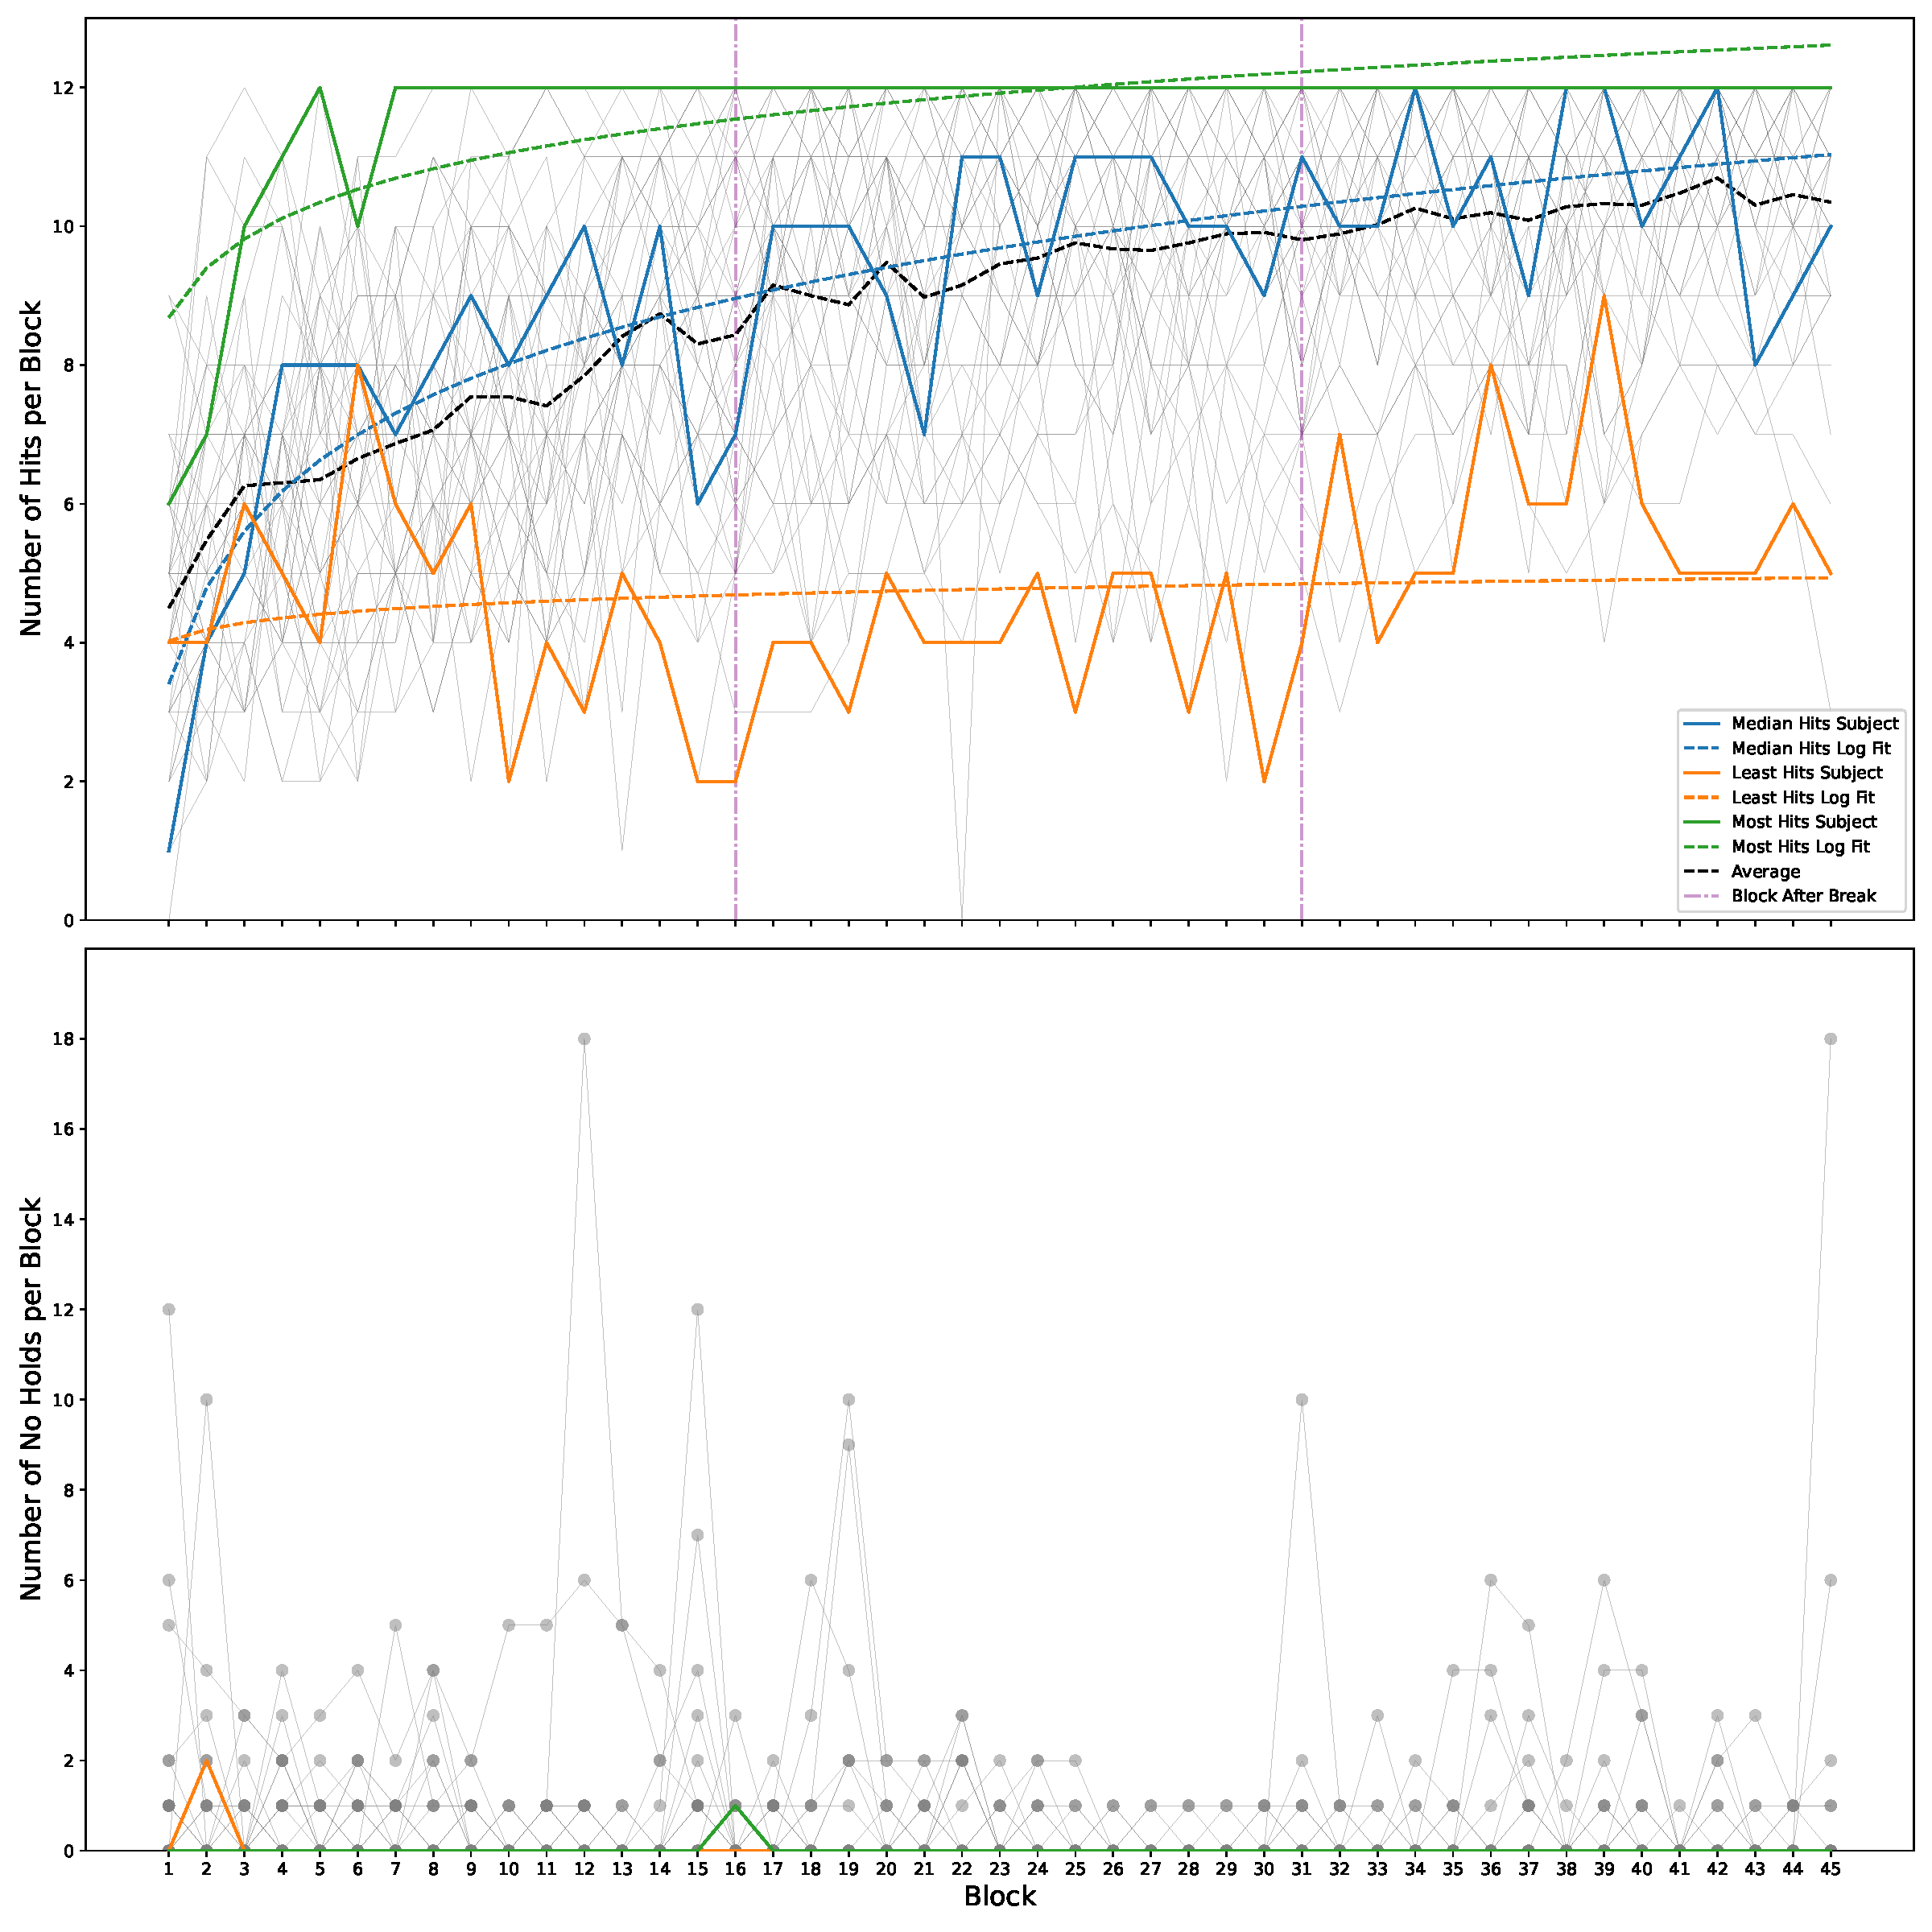
\includegraphics[width=1.3\textwidth]{analysis/hits_and_noholds_over_blocks.pdf}
%         }
%     \caption{Blah blah blah blah}\label{fig:behavior}
% \end{figure}


% \begin{figure}[H]
%     \makebox[\linewidth][c]{%
%         \centering
%         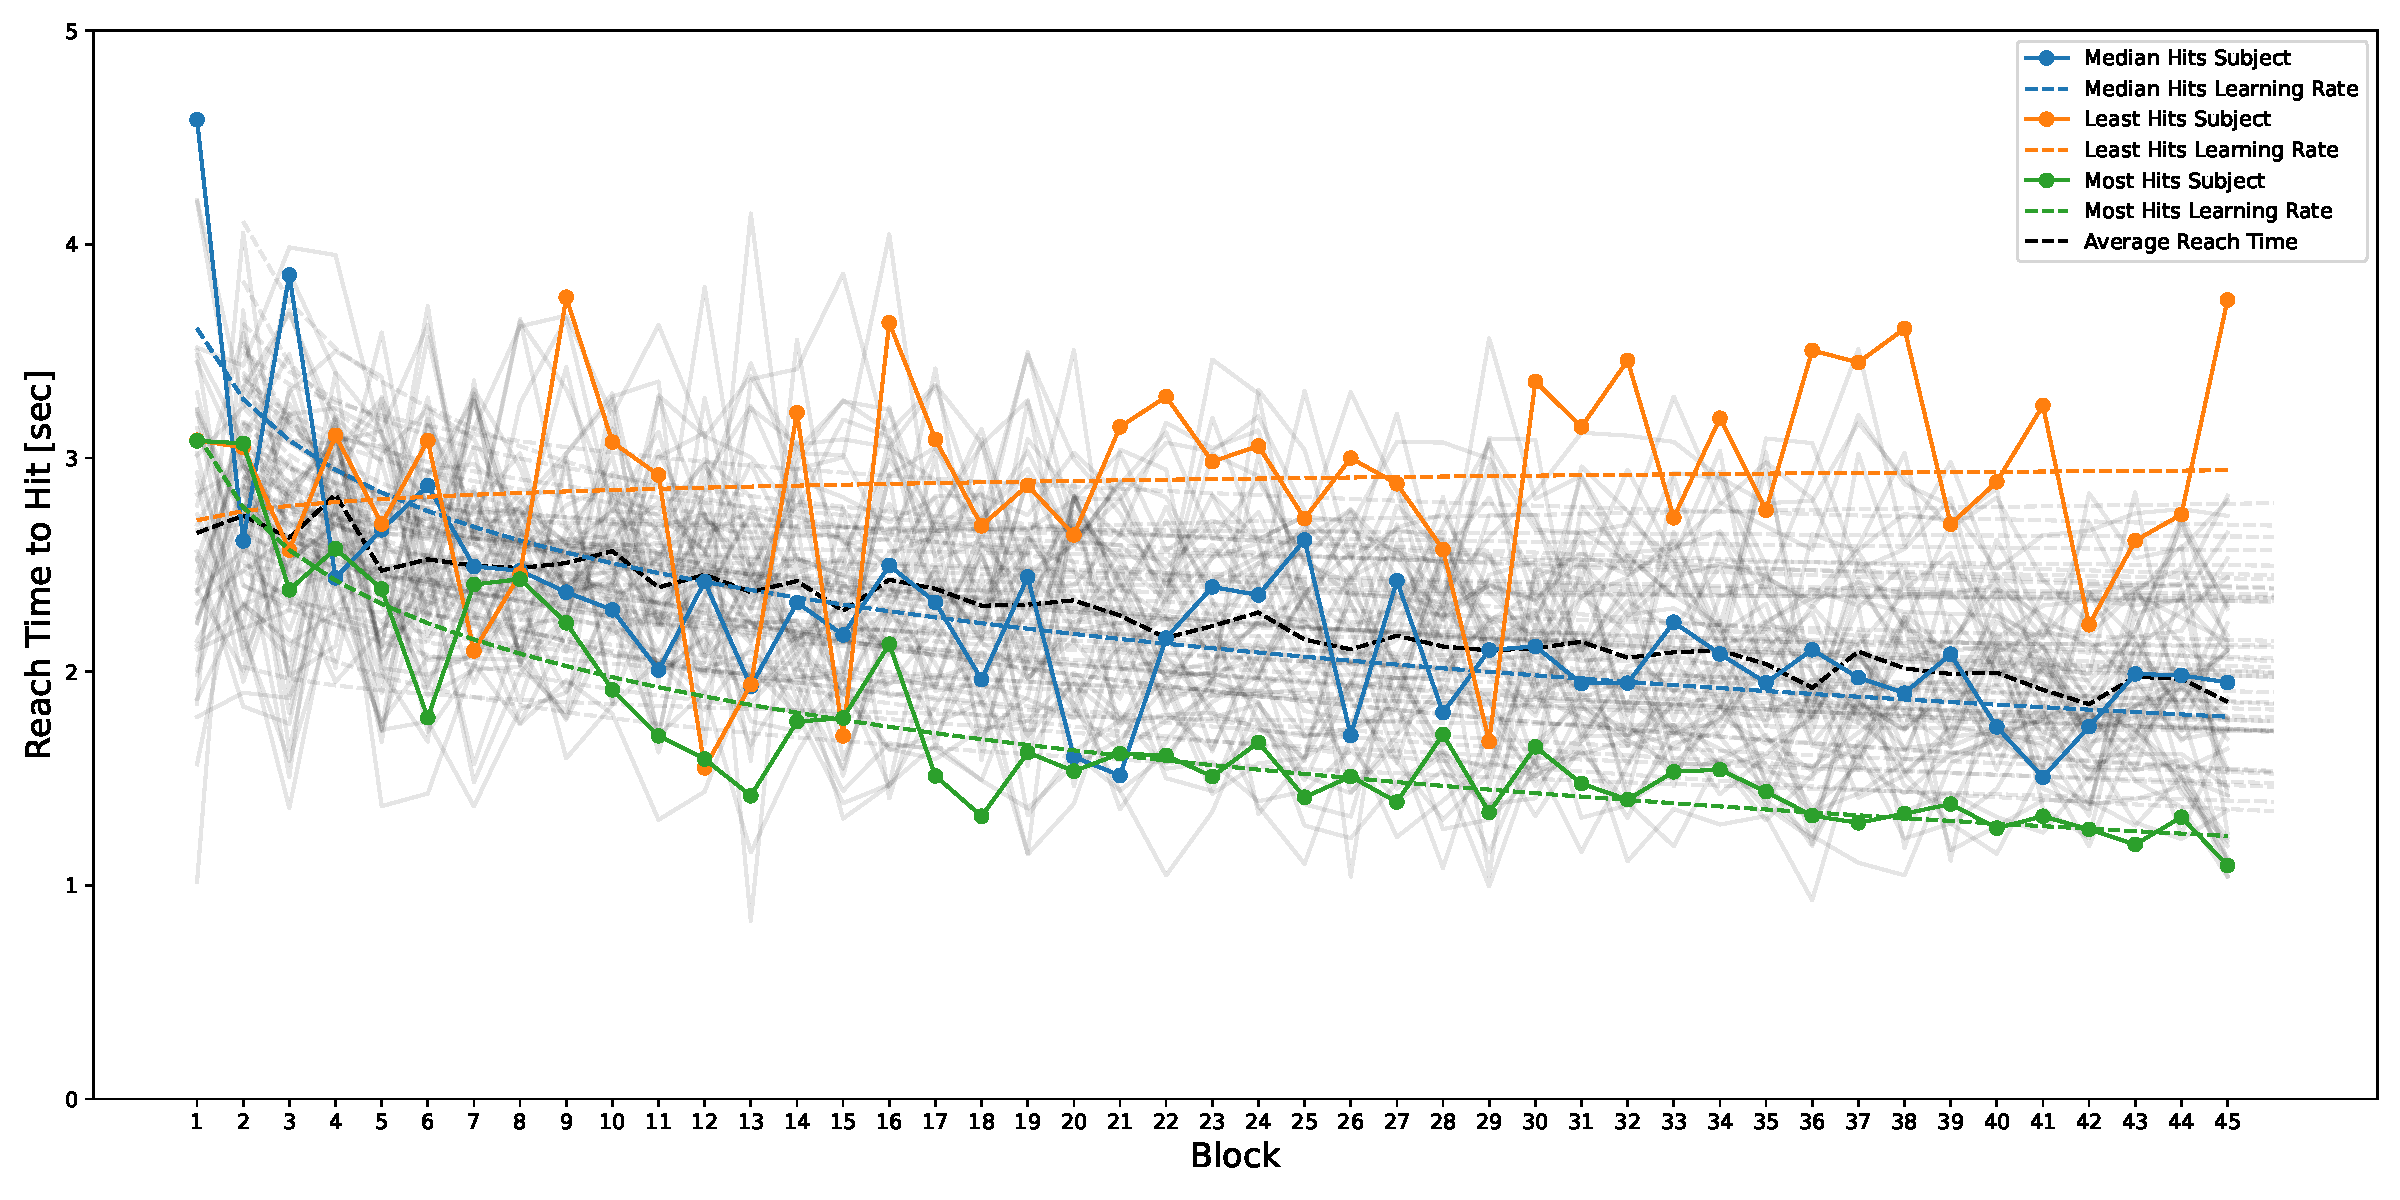
\includegraphics[width=1.3\textwidth]{analysis/reach_times_over_blocks.pdf}
%         }
%     \caption{Blah blah blah blah}\label{fig:behavior}
% \end{figure}


% \begin{figure}[H]
%     \makebox[\linewidth][c]{%
%         \centering
%         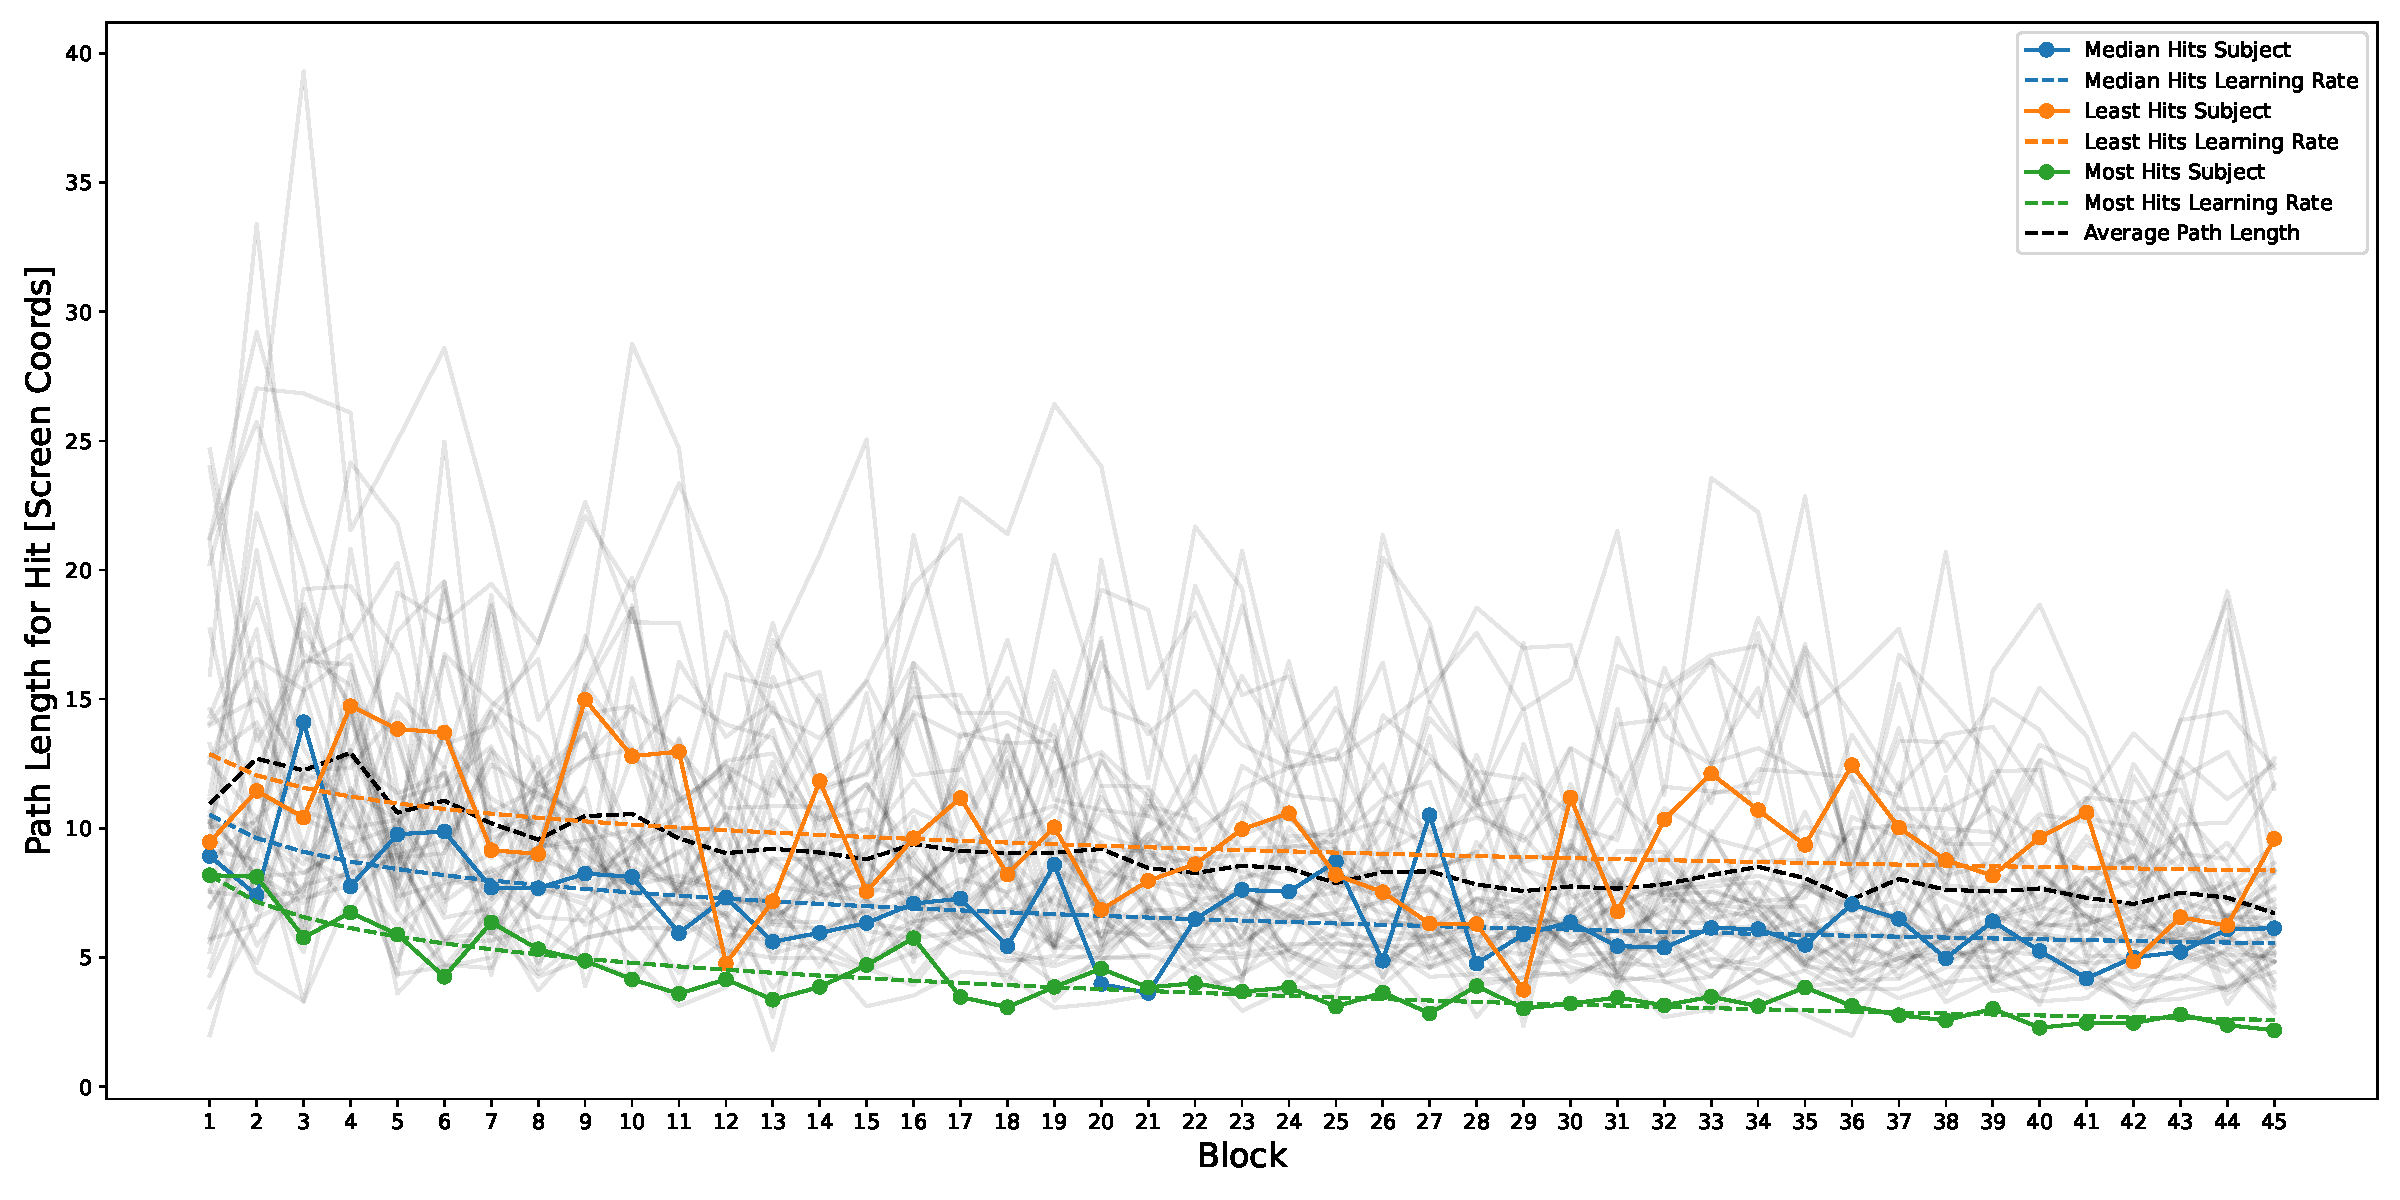
\includegraphics[width=1.3\textwidth]{analysis/path_length_over_blocks.pdf}
%         }
%     \caption{Blah blah blah blah}\label{fig:behavior}
% \end{figure}


% \begin{figure}[H]
%     \makebox[\linewidth][c]{%
%         \centering
%         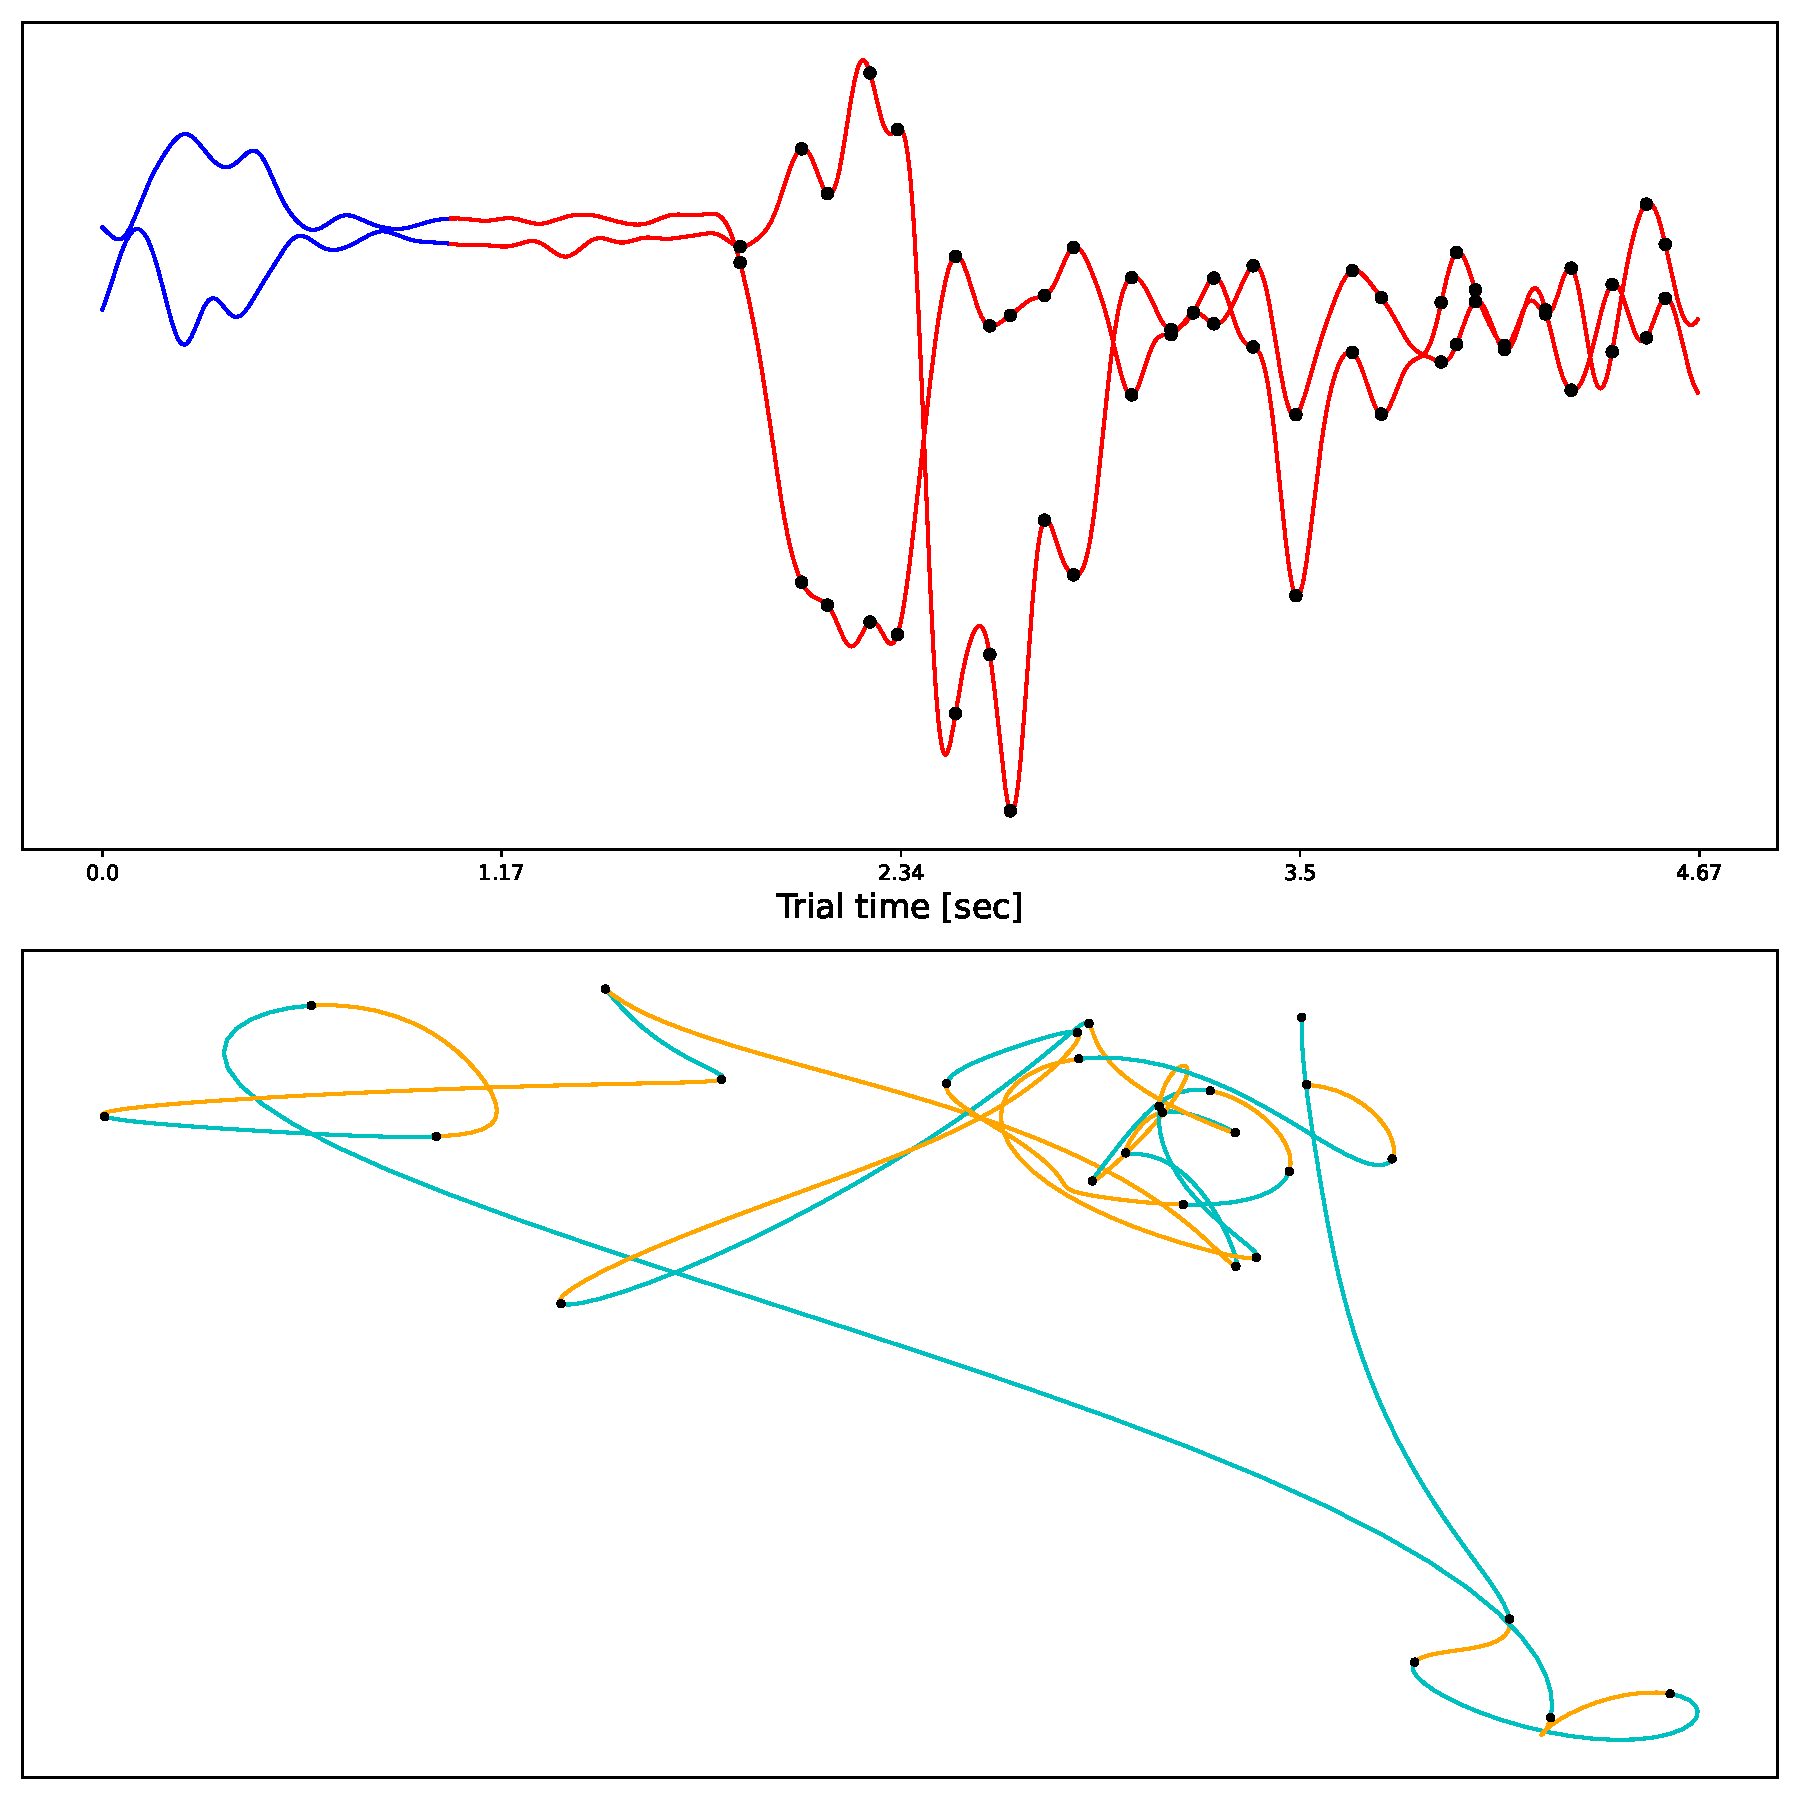
\includegraphics[width=\textwidth]{analysis/example_path_segments.pdf}
%     }
%     \caption{Blah blah blah blah}\label{fig:behavior}
%     \end{figure}


% \begin{figure}[H]
%     \makebox[\linewidth][c]{%
%         \centering
%         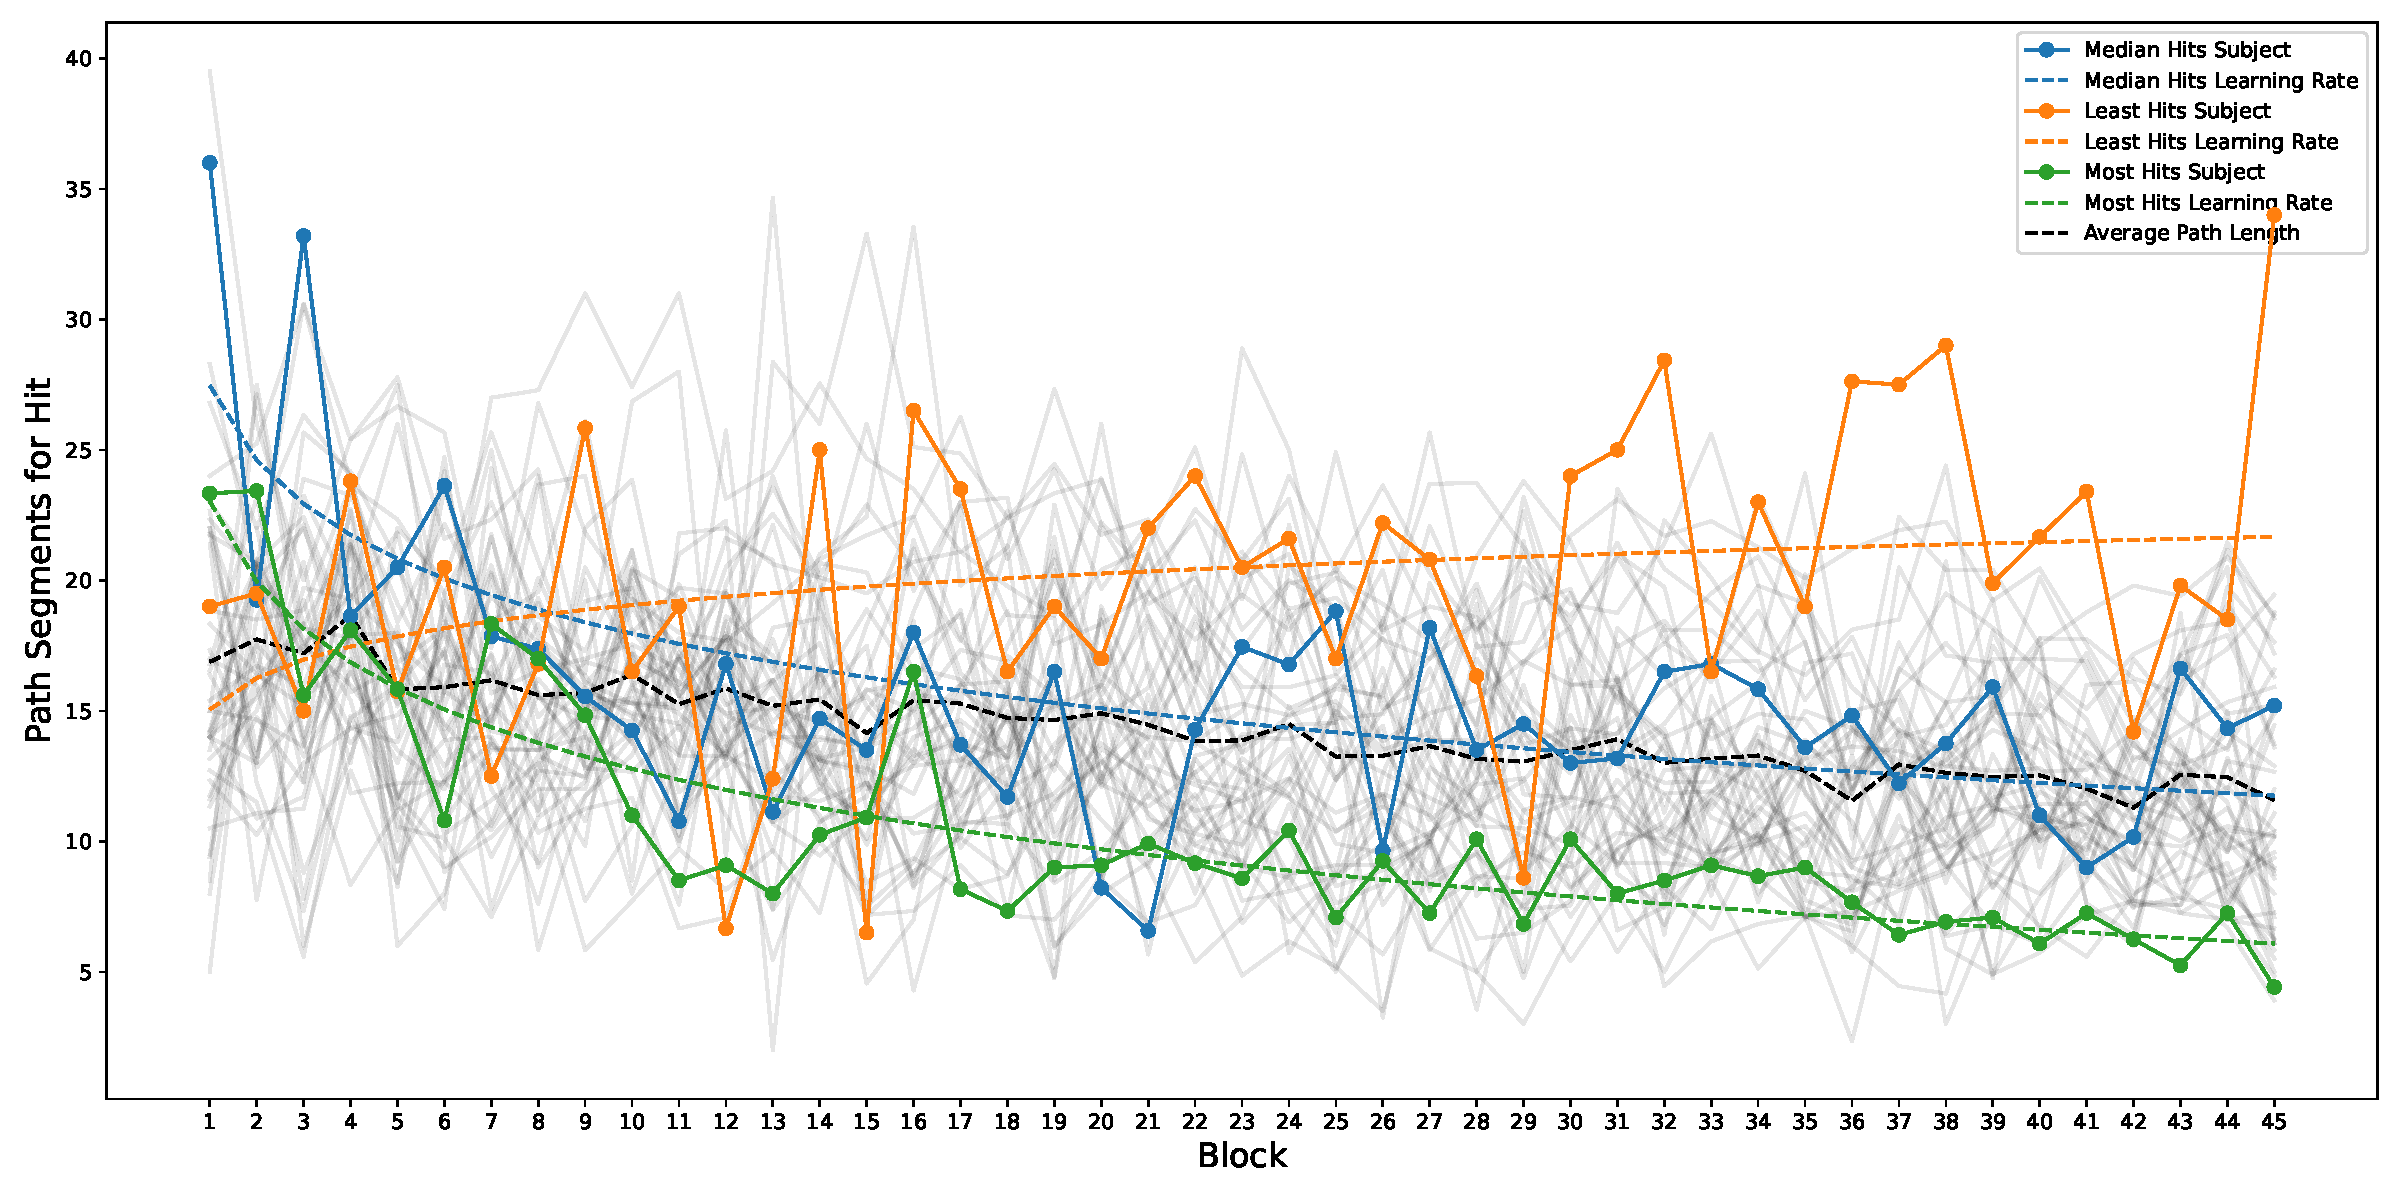
\includegraphics[width=1.3\textwidth]{analysis/segments_over_blocks.pdf}
%     }
%     \caption{Blah blah blah blah}\label{fig:behavior}
% \end{figure}


% \begin{figure}[H]
%     \makebox[\linewidth][c]{%
%         \centering
%         \begin{subfigure}{.5\textwidth}
%             \centering
%             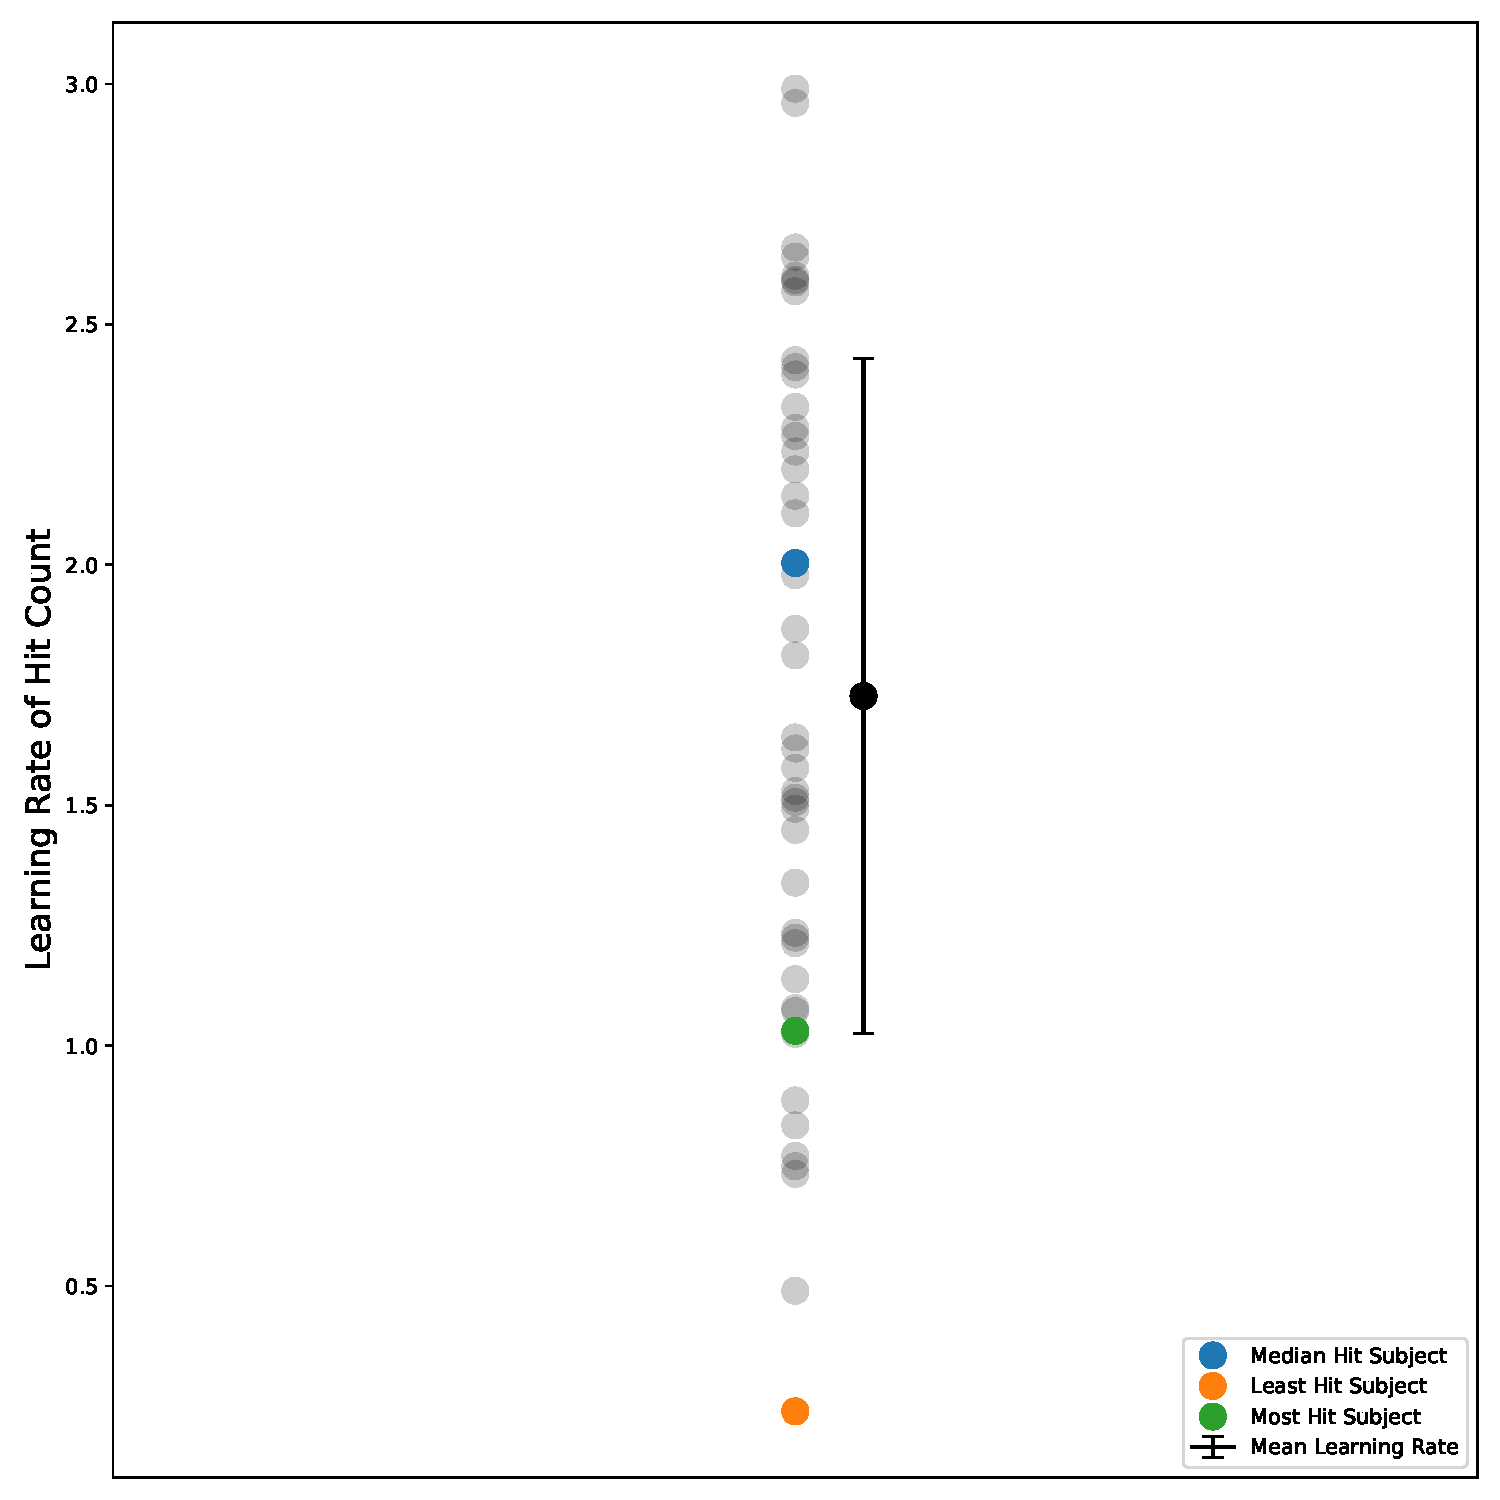
\includegraphics[width=\textwidth]{analysis/hits_learning_rates.pdf}
%             \caption{}
%             \label{fig:hit_learning_rates}
%         \end{subfigure}%
%         \begin{subfigure}{.5\textwidth}
%             \centering
%             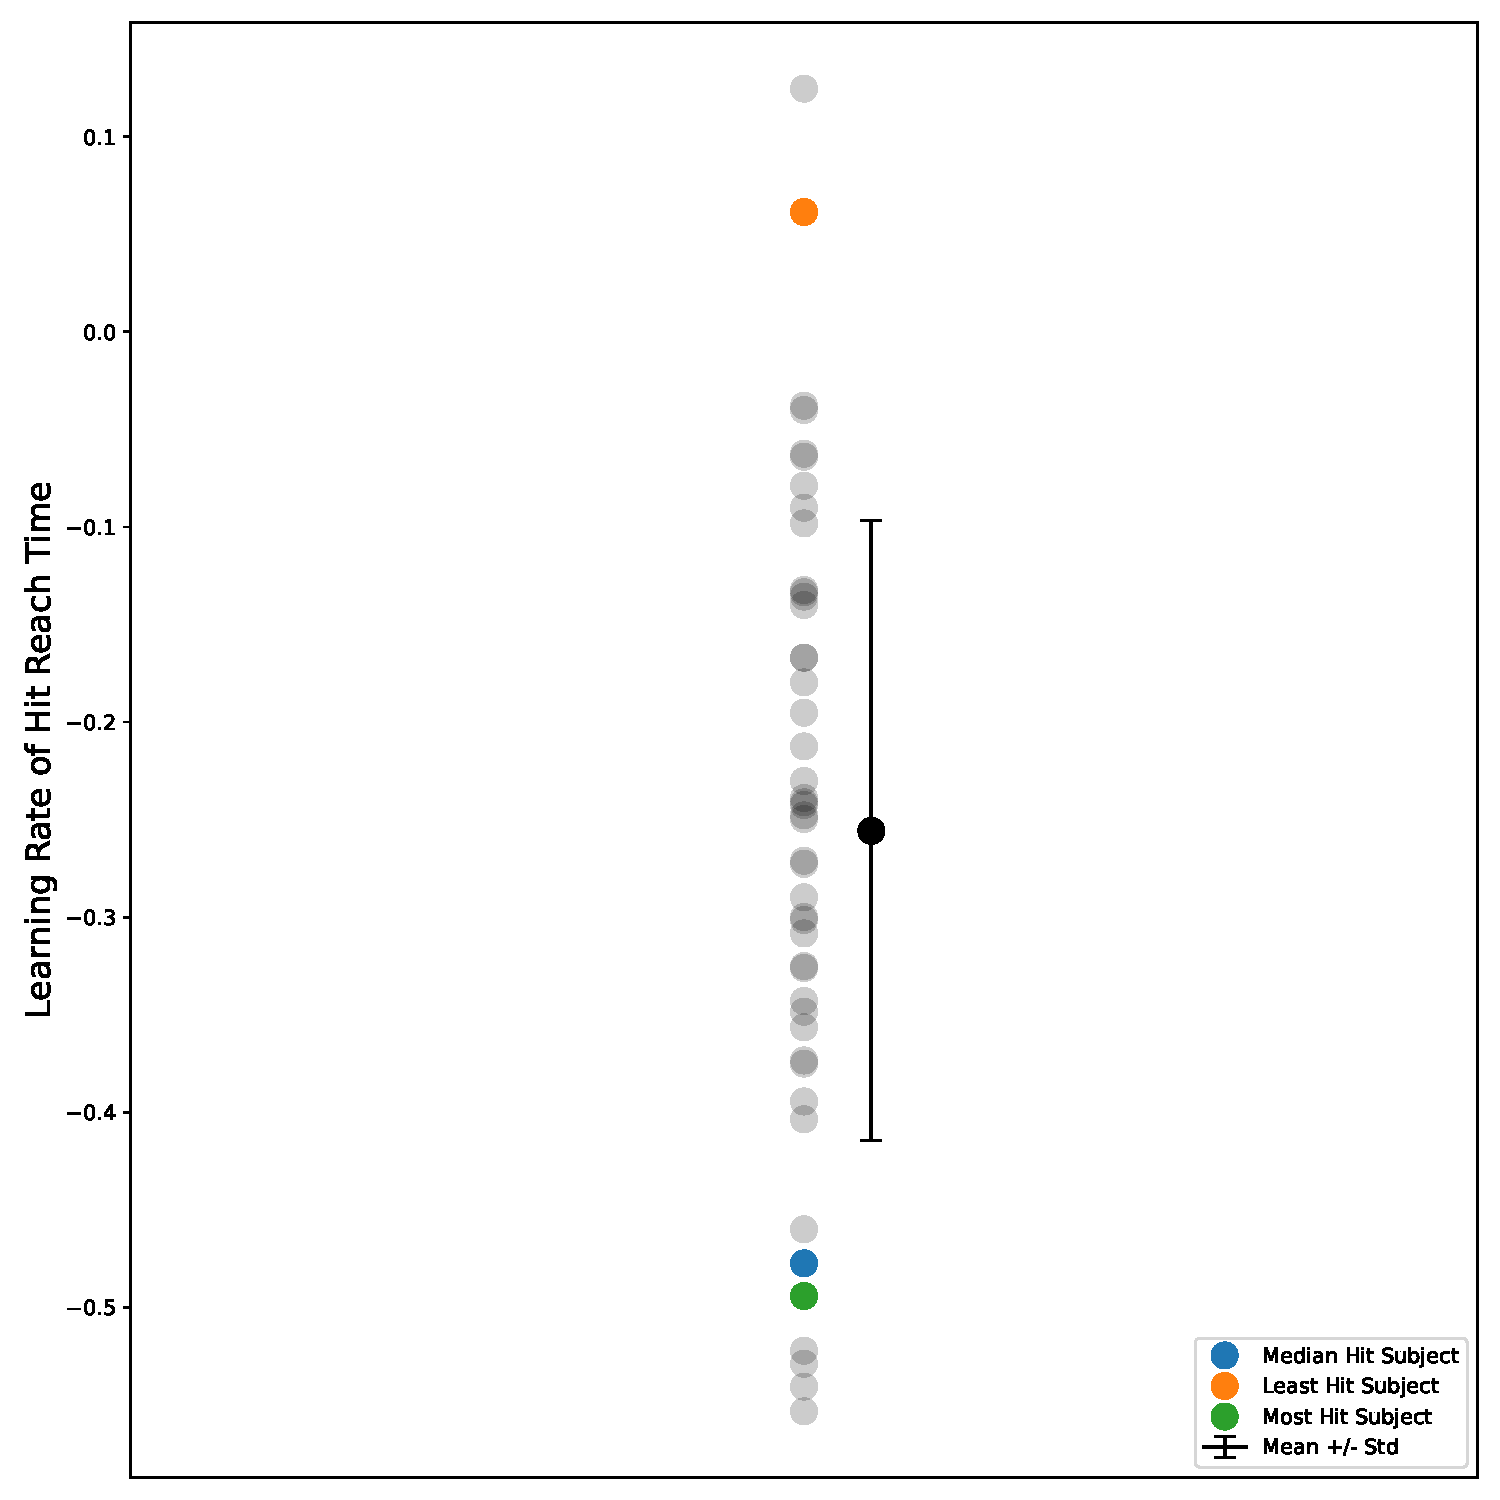
\includegraphics[width=\textwidth]{analysis/reach_time_learning_rates.pdf}
%             \caption{}            
%             \label{fig:reach_time_learning_rates}
%         \end{subfigure}%
%     }

%     \makebox[\linewidth][c]{%
%         \begin{subfigure}{.5\textwidth}
%             \centering
%             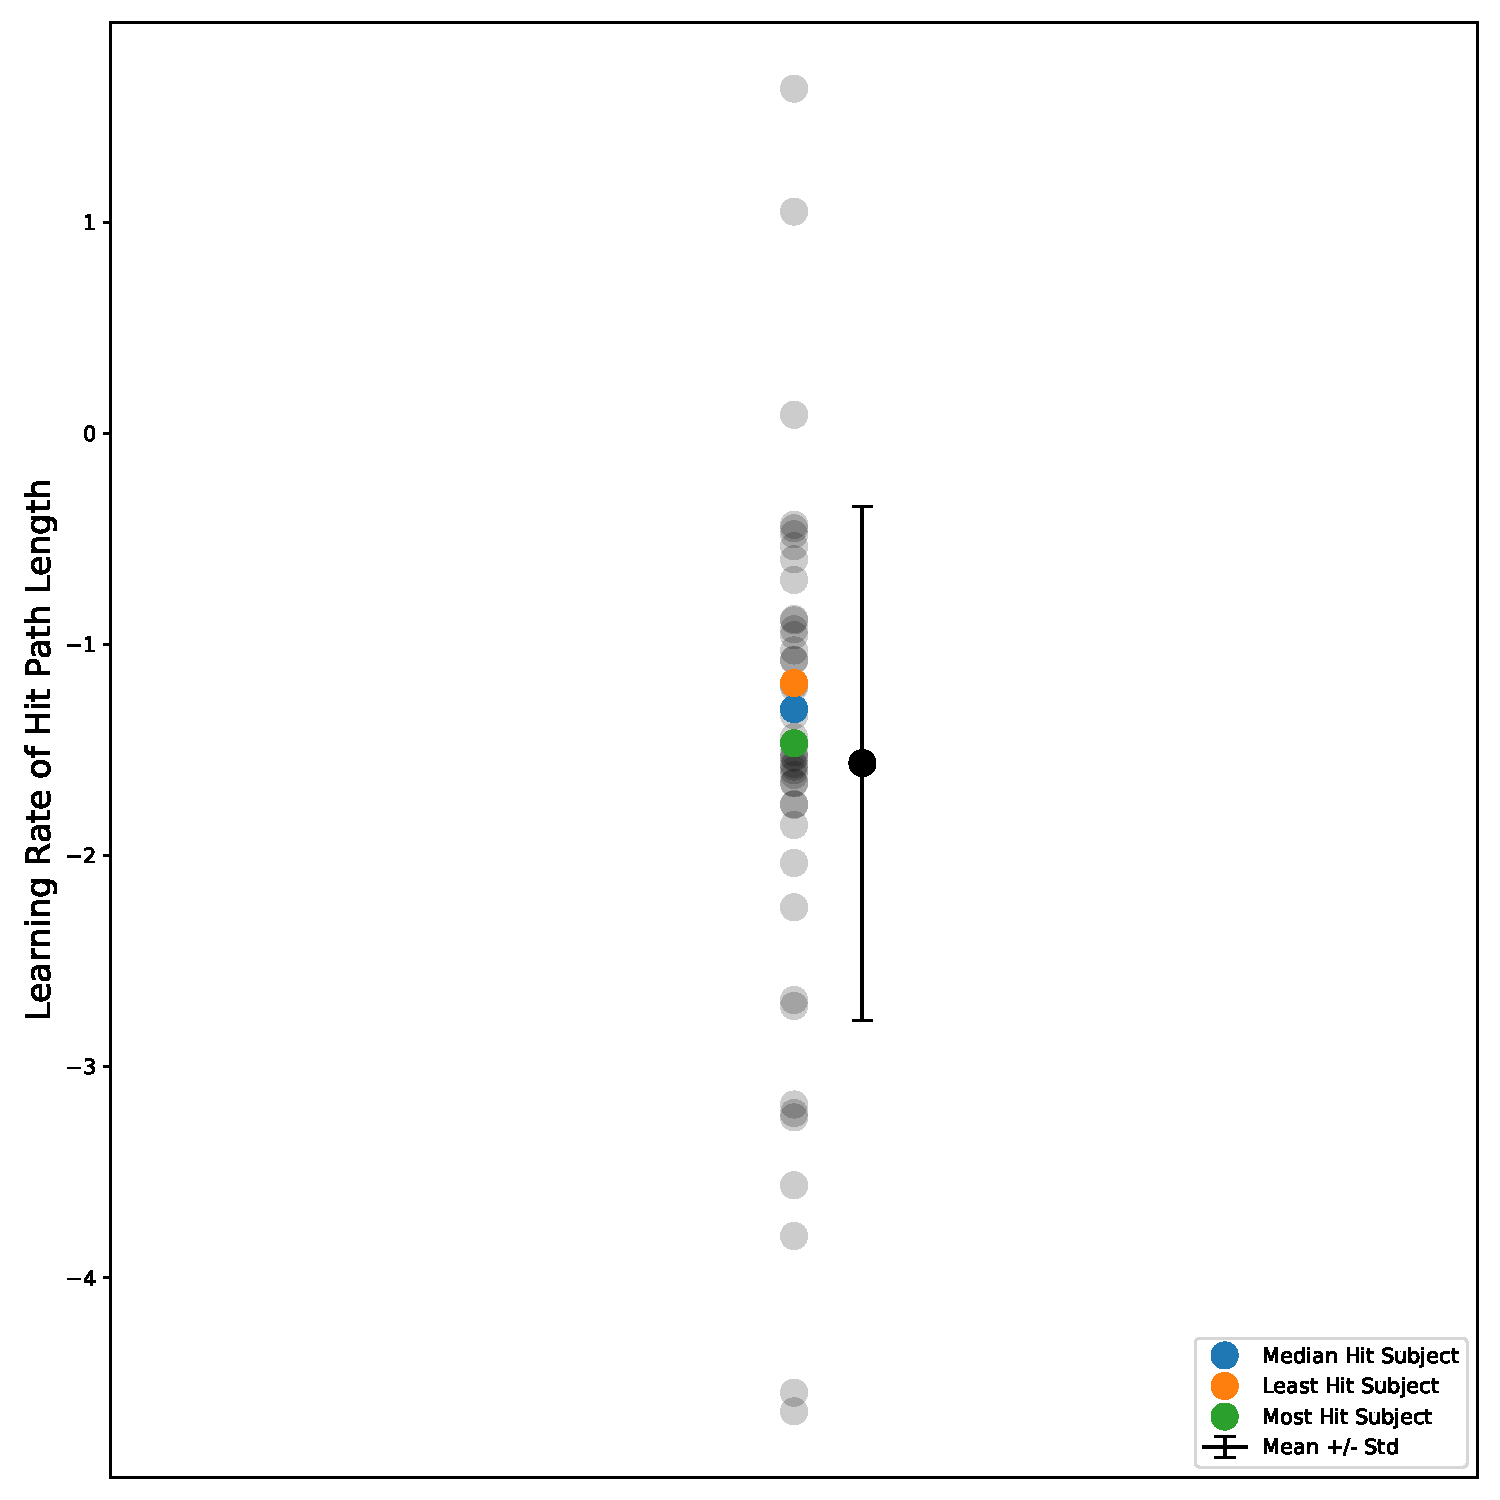
\includegraphics[width=\textwidth]{analysis/path_length_learning_rates.pdf}
%             \caption{}            
%             \label{fig:path_length_learning_rates}
%         \end{subfigure}
%         \begin{subfigure}{.5\textwidth}
%             \centering
%             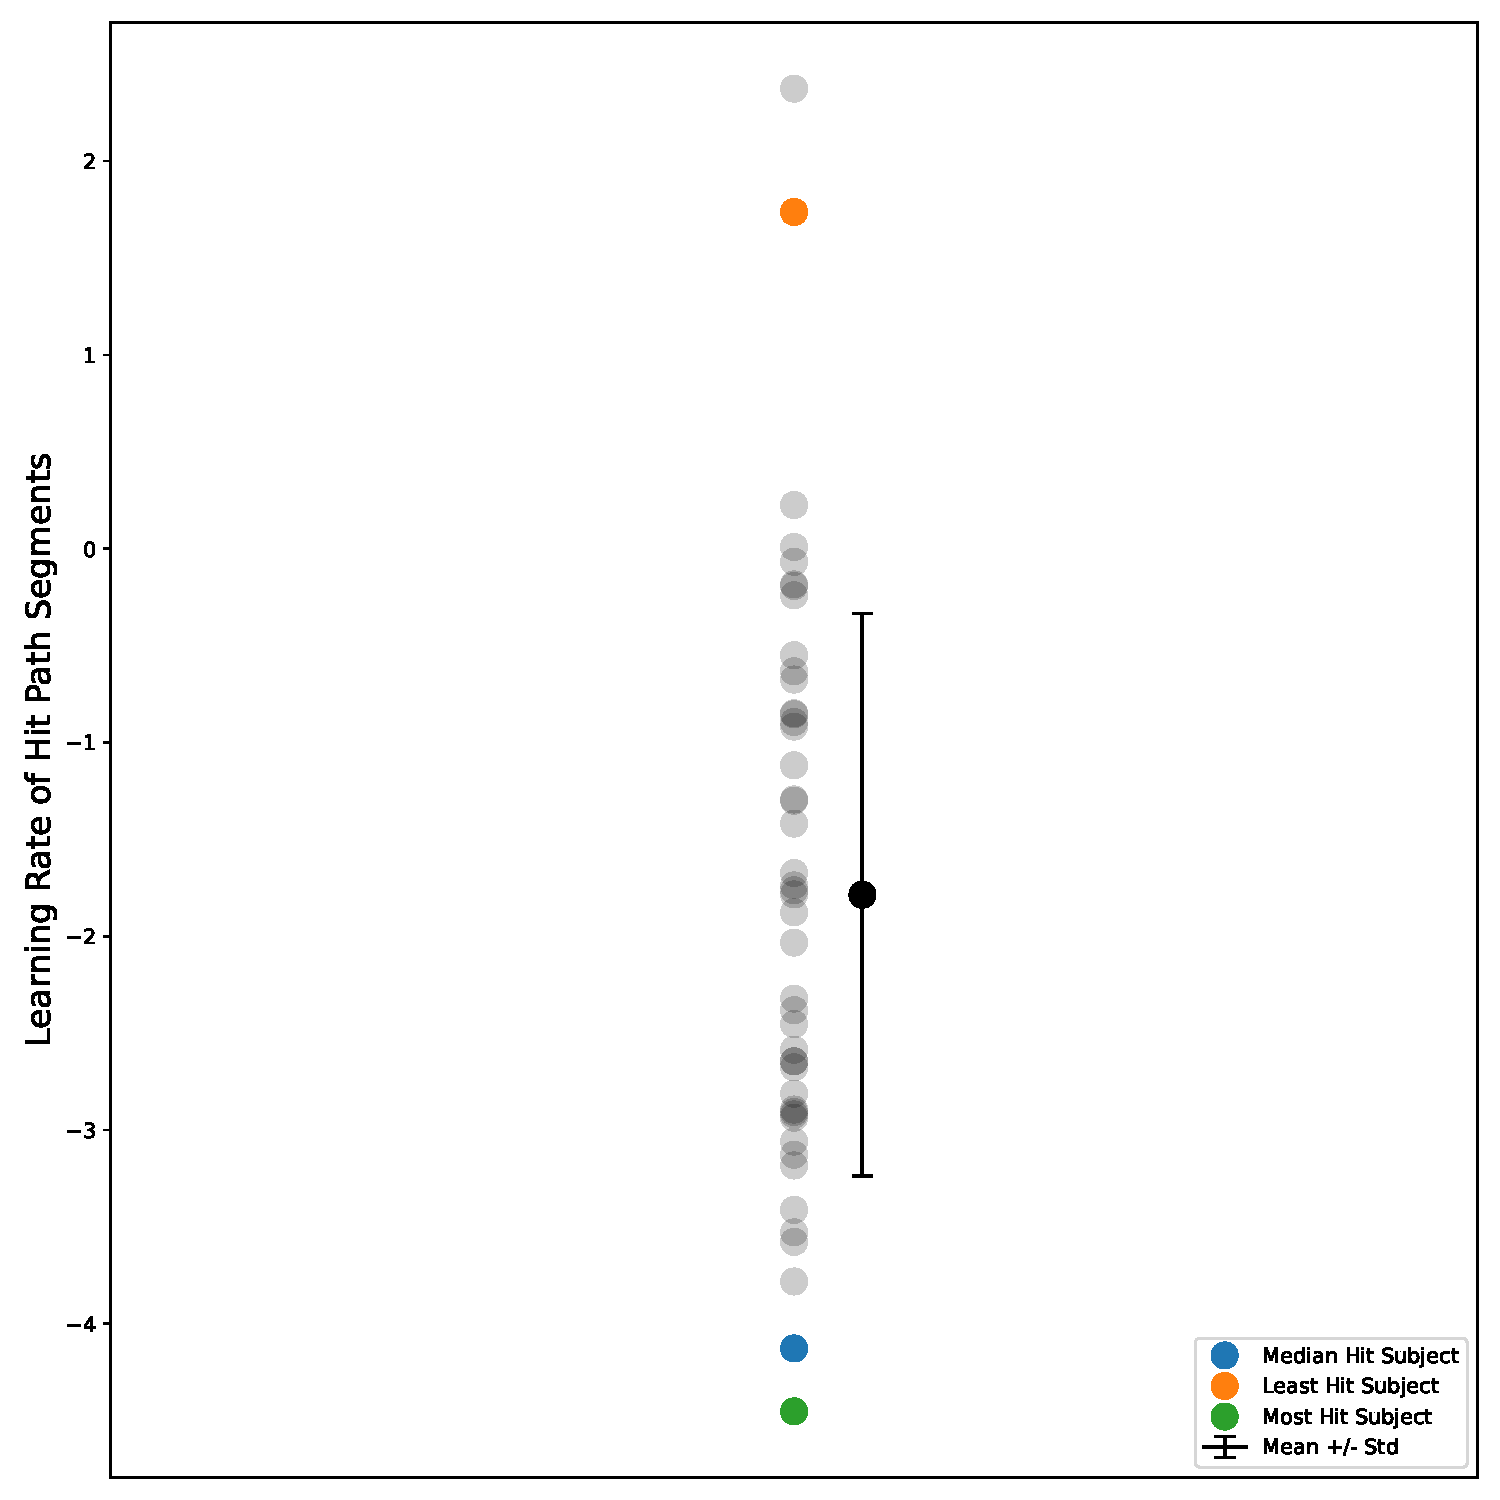
\includegraphics[width=\textwidth]{analysis/segment_learning_rates.pdf}
%             \caption{}            
%             \label{fig:path_length_learning_rates}
%         \end{subfigure}
%     }
%     \caption{Learning rates for different measures of performance}
%     \label{fig:three graphs}
% \end{figure}


% \begin{figure}[H]
%     \makebox[\linewidth][c]{%
%         \centering
%         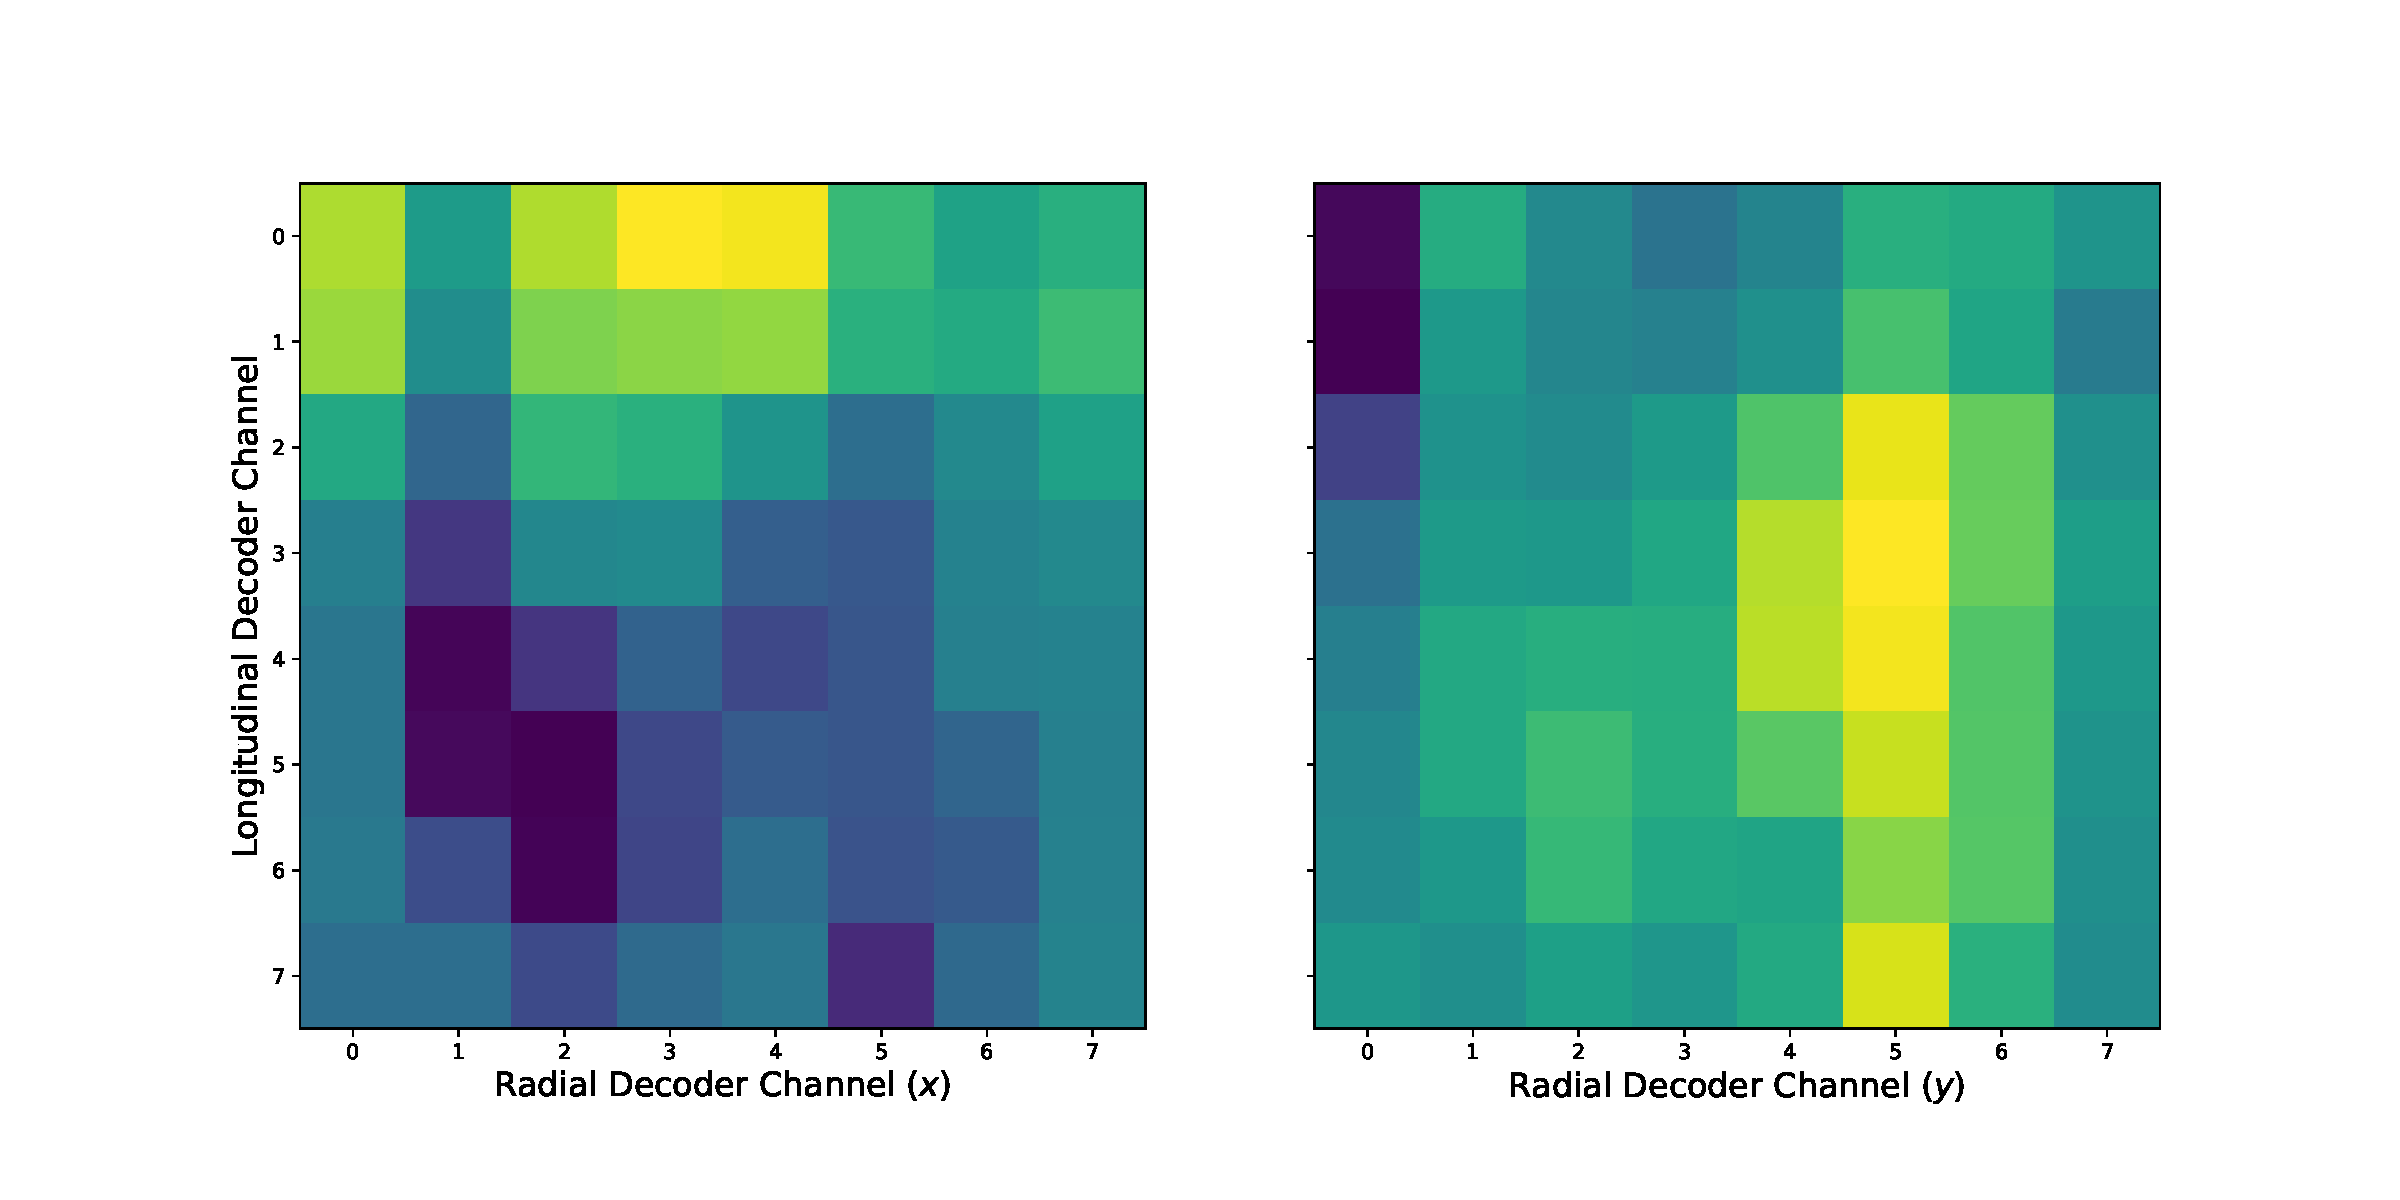
\includegraphics[width=1.4\textwidth]{analysis/example_decoder.pdf}
%     }
%     \caption{Blah blah blah blah}\label{fig:behavior}
% \end{figure}


% \begin{figure}[H]
%     \makebox[\linewidth][c]{%
%         \centering
%         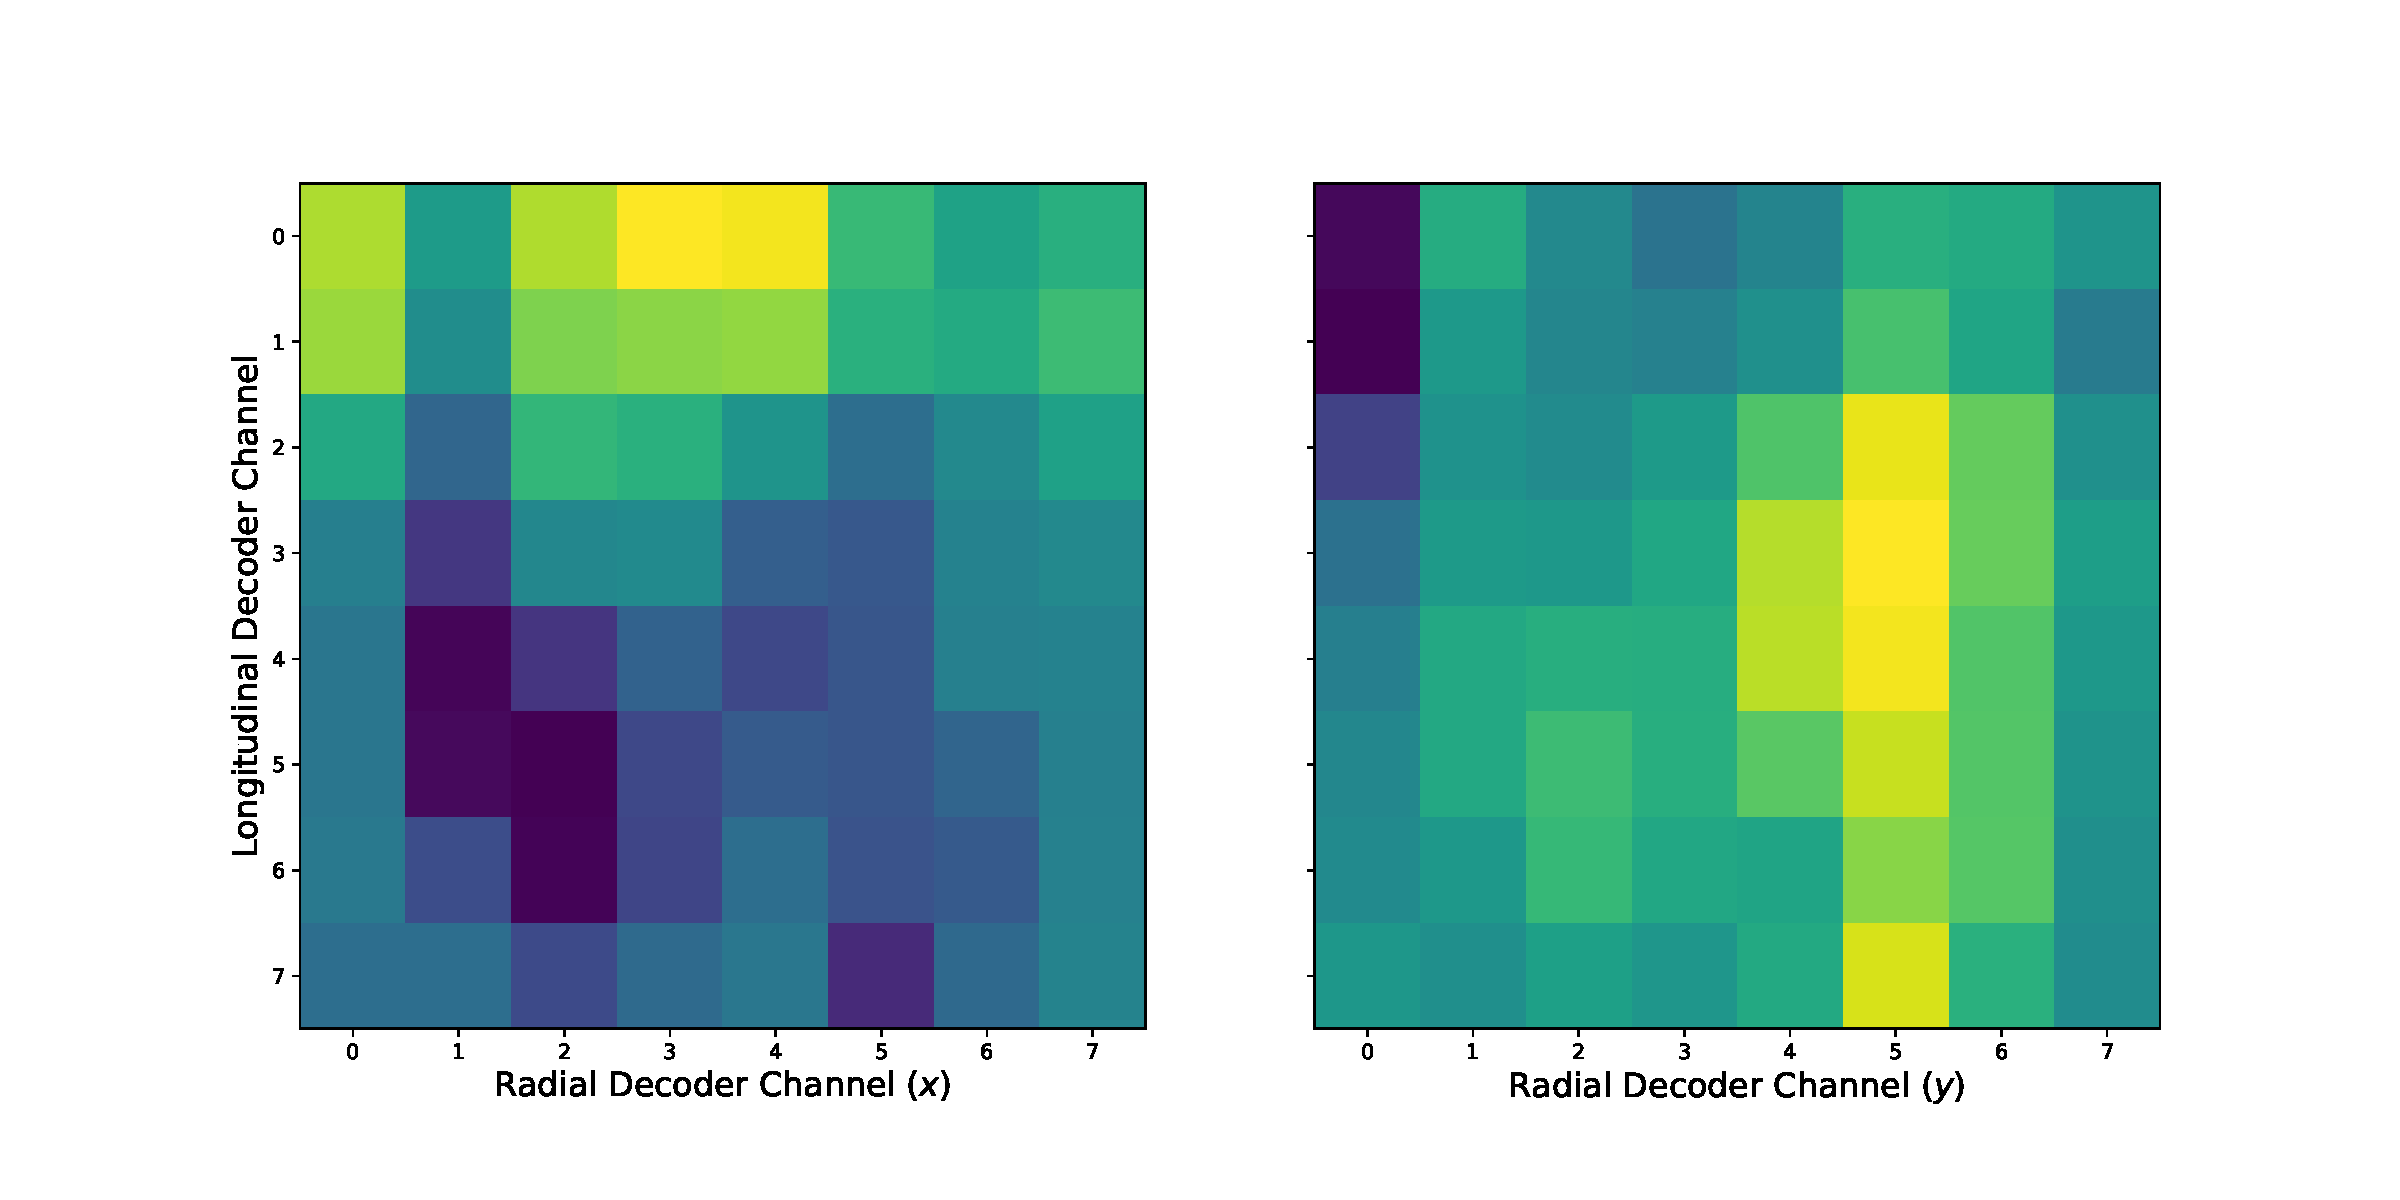
\includegraphics[width=1.4\textwidth]{analysis/example_decoder.pdf}
%     }
%     \caption{Blah blah blah blah}\label{fig:behavior}
% \end{figure}


% \begin{figure}[H]
%     \makebox[\linewidth][c]{%
%         \centering
%         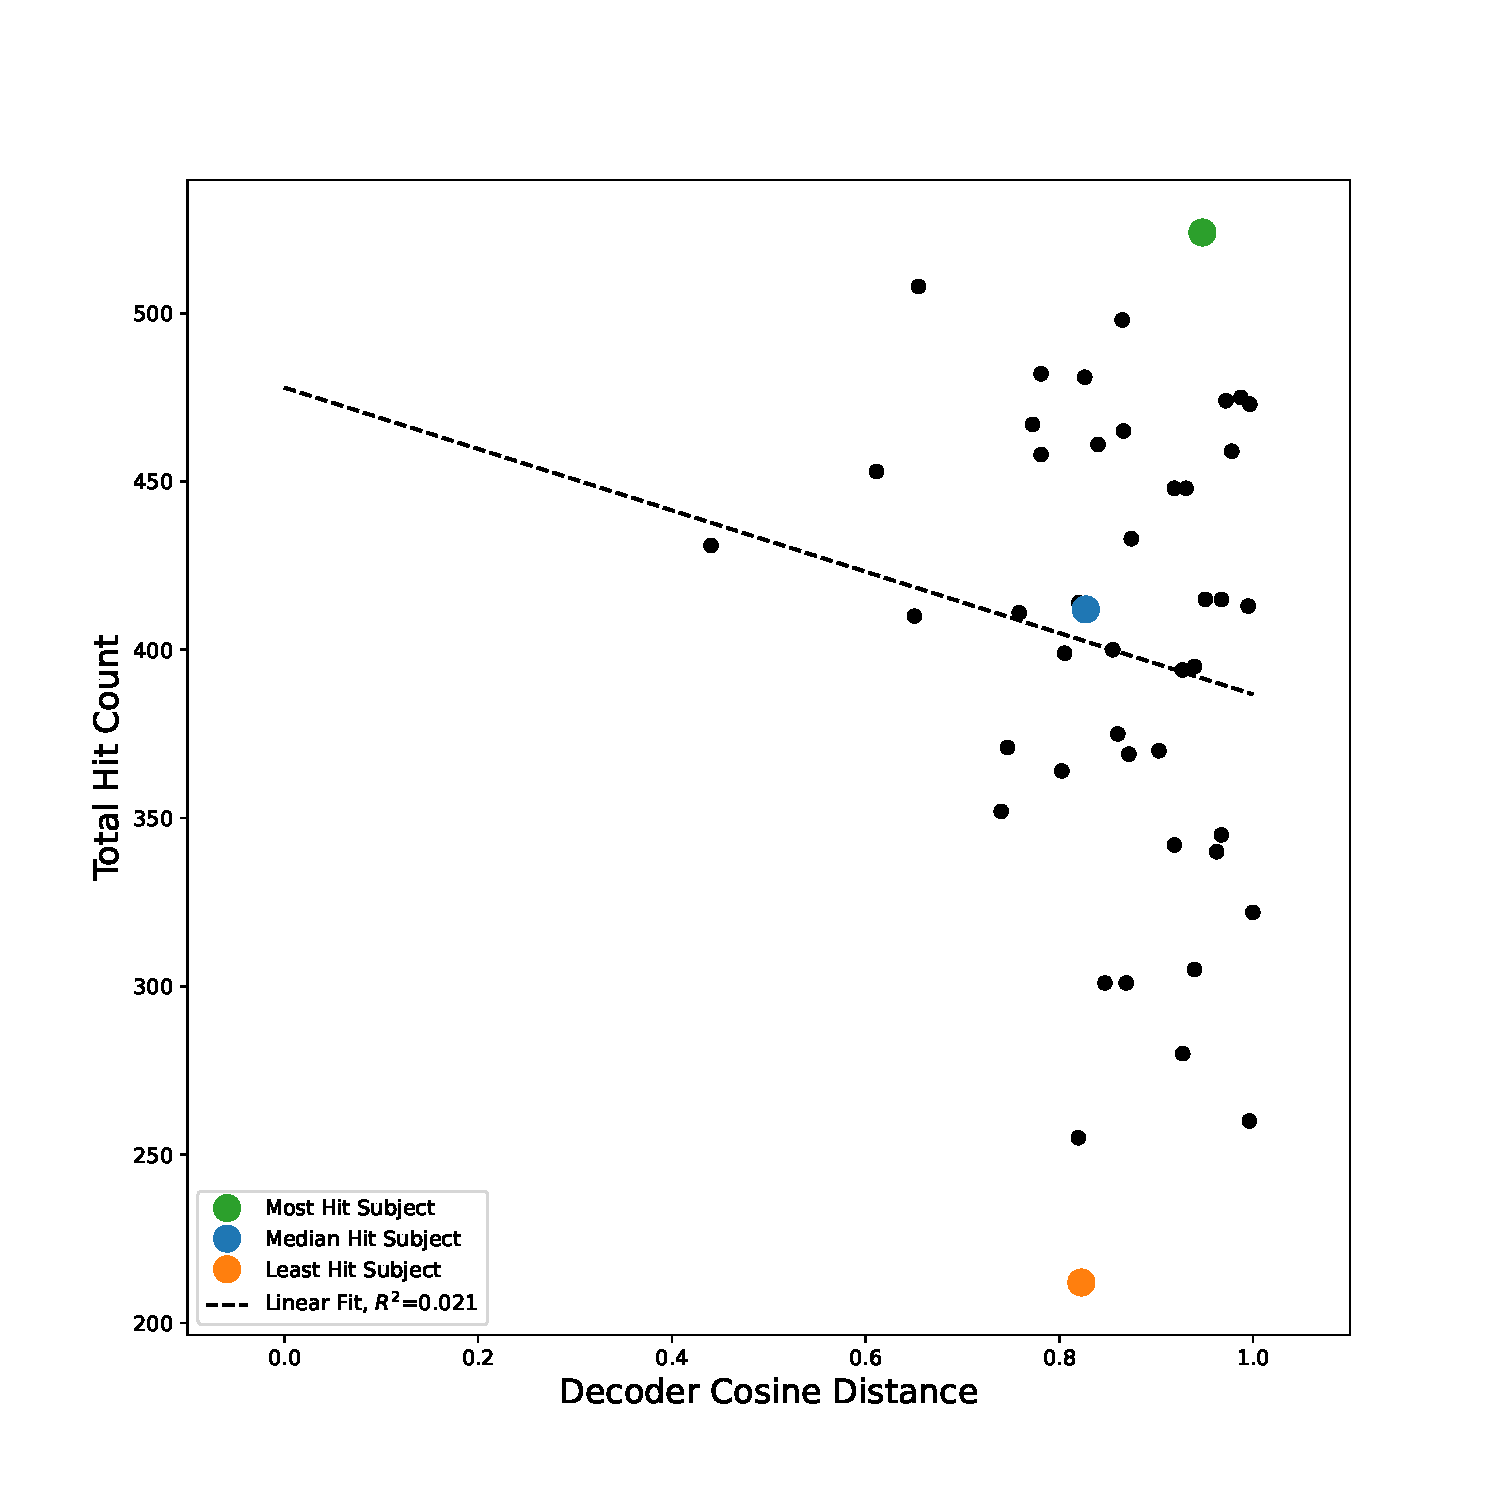
\includegraphics[width=.75\textwidth]{analysis/hit_count_decoder_cosine.pdf}
%     }
%     \caption{Blah blah blah blah}\label{fig:behavior}
% \end{figure}


% \begin{figure}[H]
%     \makebox[\linewidth][c]{%
%         \centering
%         \begin{subfigure}{0.7\textwidth}
%             \centering
%             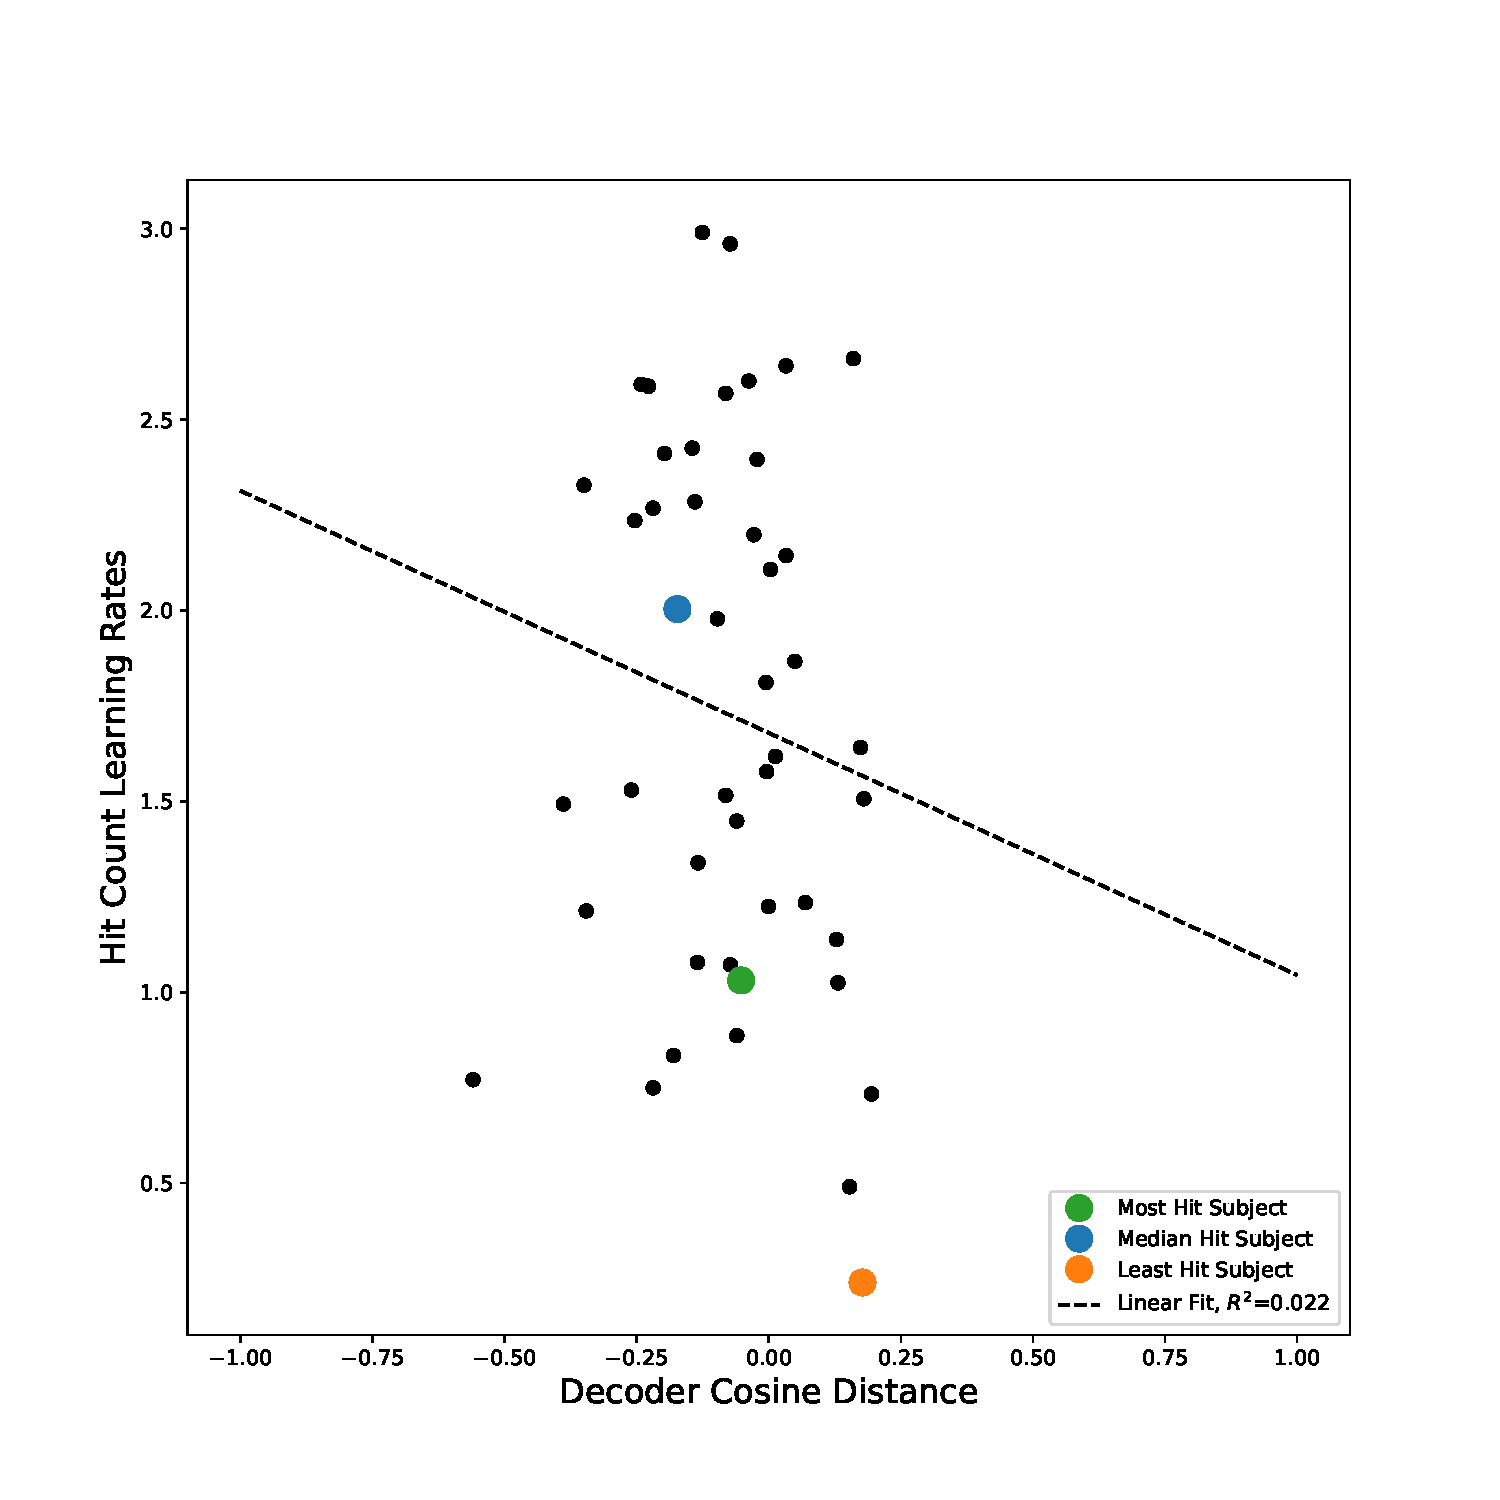
\includegraphics[width=\textwidth]{analysis/hit_lr_decoder_cosine.pdf}
%             \caption{}
%             \label{fig:hit_learning_rates}
%         \end{subfigure}%
%         \begin{subfigure}{0.7\textwidth}
%             \centering
%             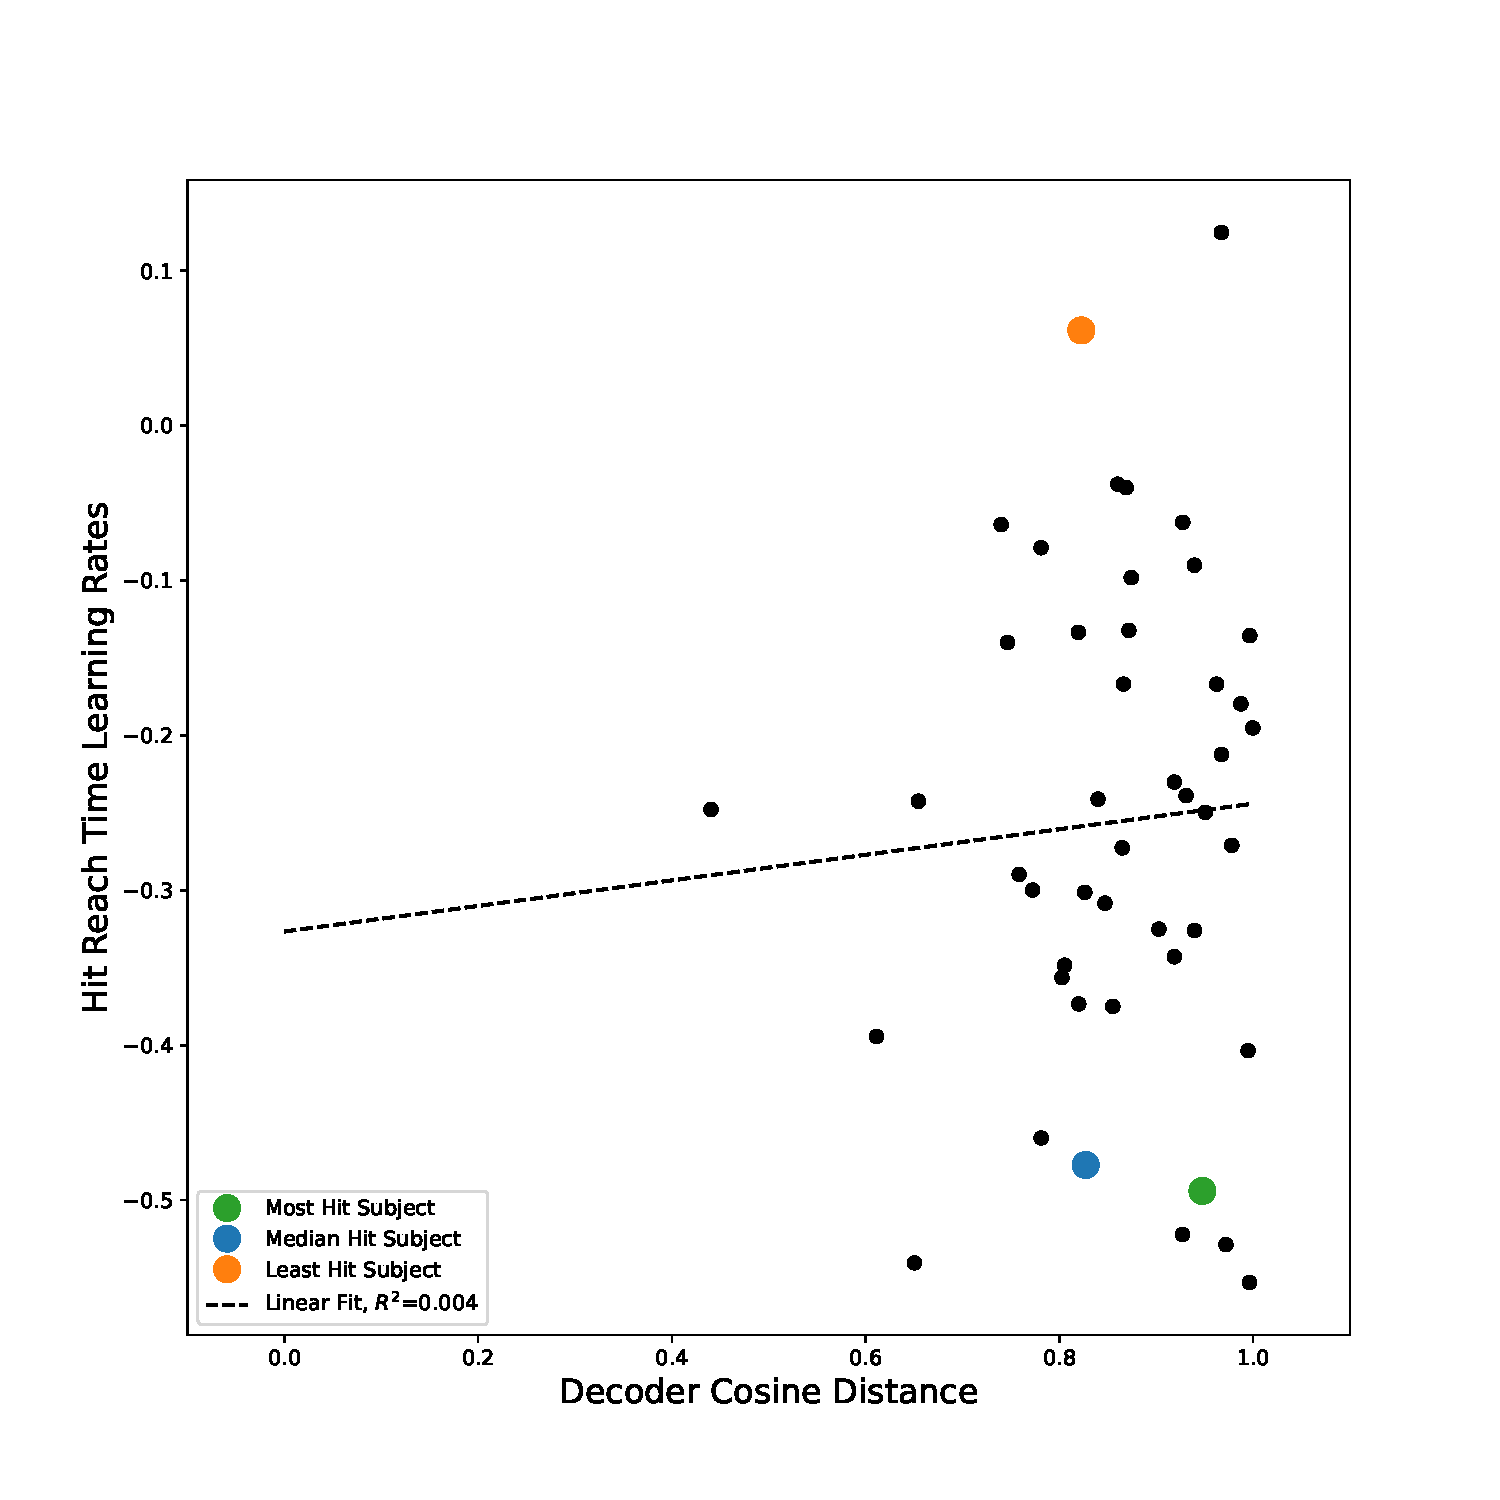
\includegraphics[width=\textwidth]{analysis/reach_time_lr_decoder_cosine.pdf}
%             \caption{}            
%             \label{fig:reach_time_learning_rates}
%         \end{subfigure}
%     }

%     \makebox[\linewidth][c]{%
%         \begin{subfigure}{0.7\textwidth}
%             \centering
%             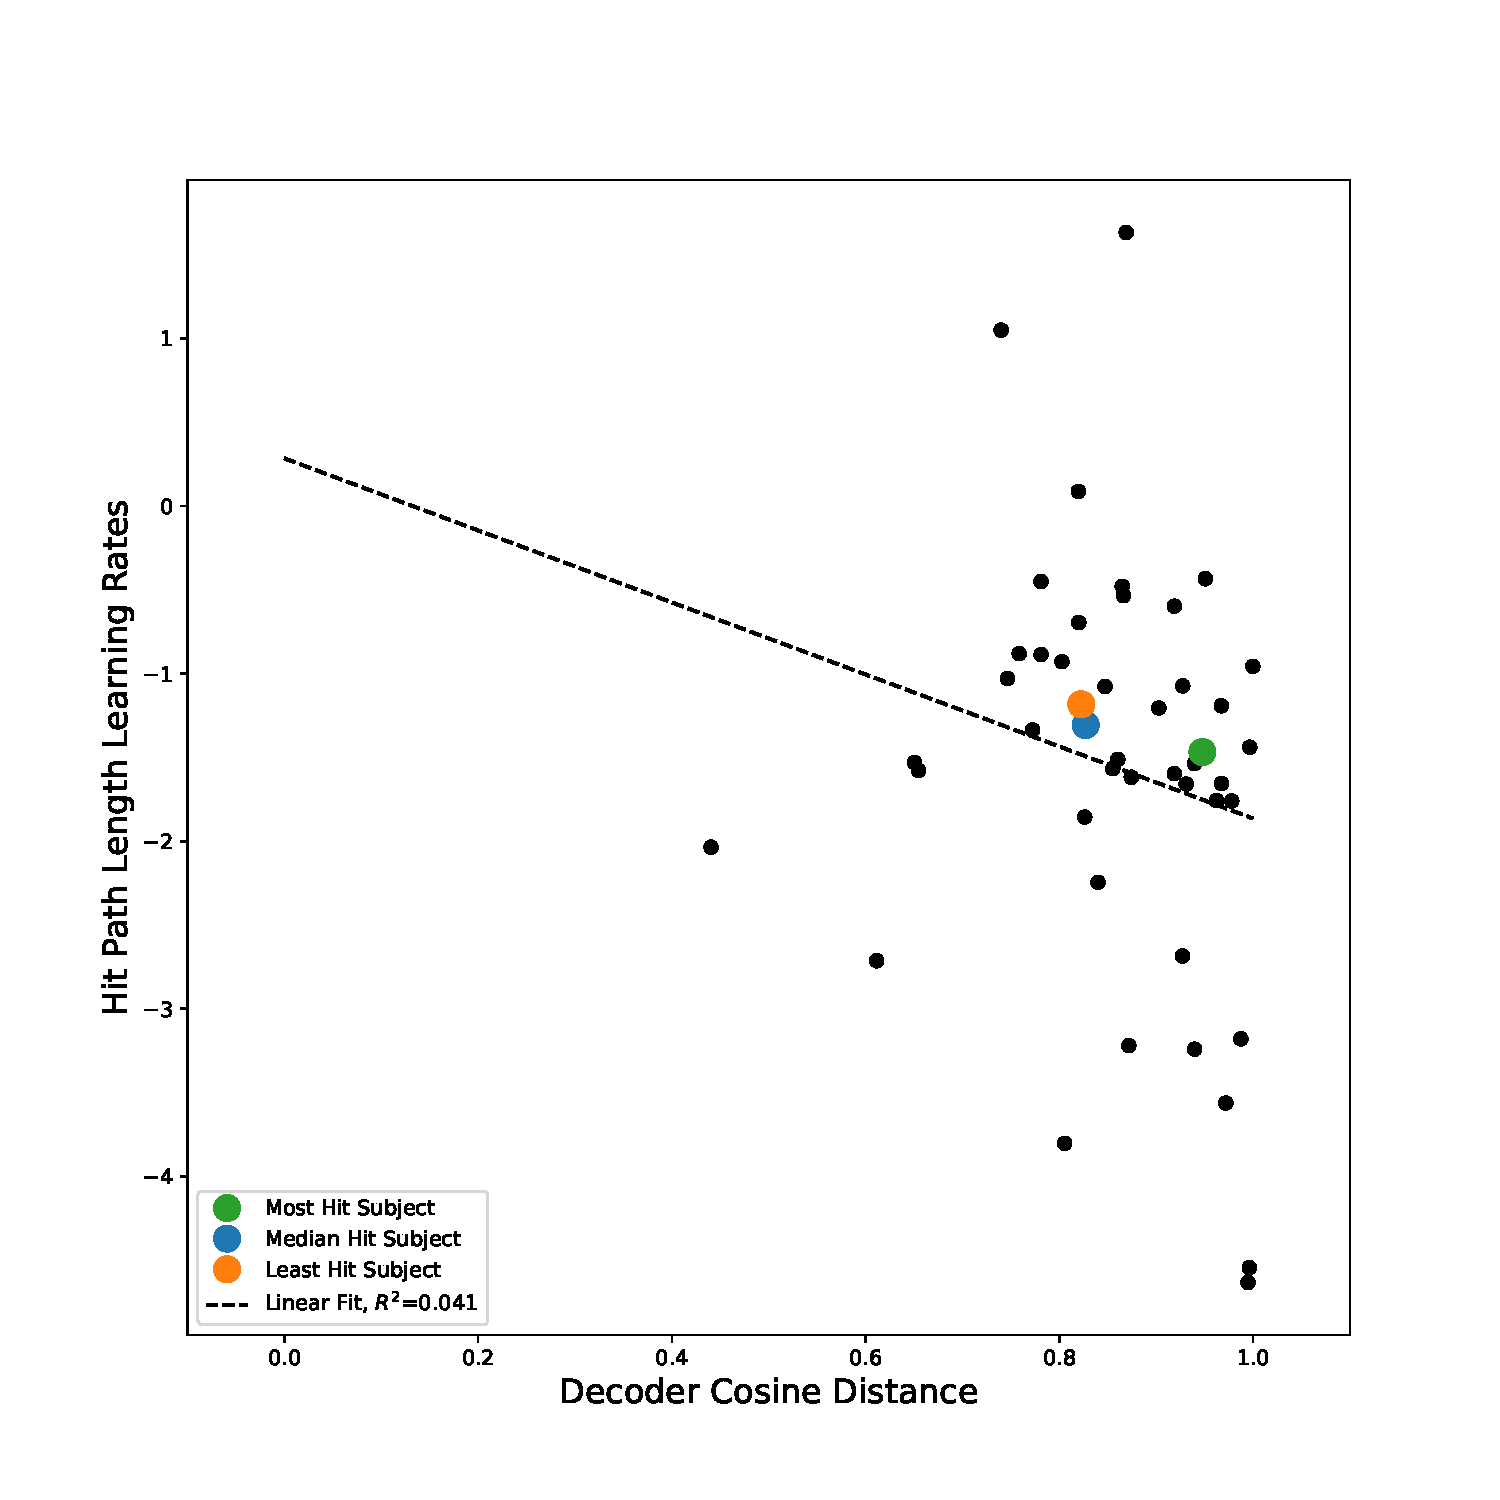
\includegraphics[width=\textwidth]{analysis/path_length_lr_decoder_cosine.pdf}
%             \caption{}            
%             \label{fig:path_length_learning_rates}
%         \end{subfigure}%
%         \begin{subfigure}{0.7\textwidth}
%             \centering
%             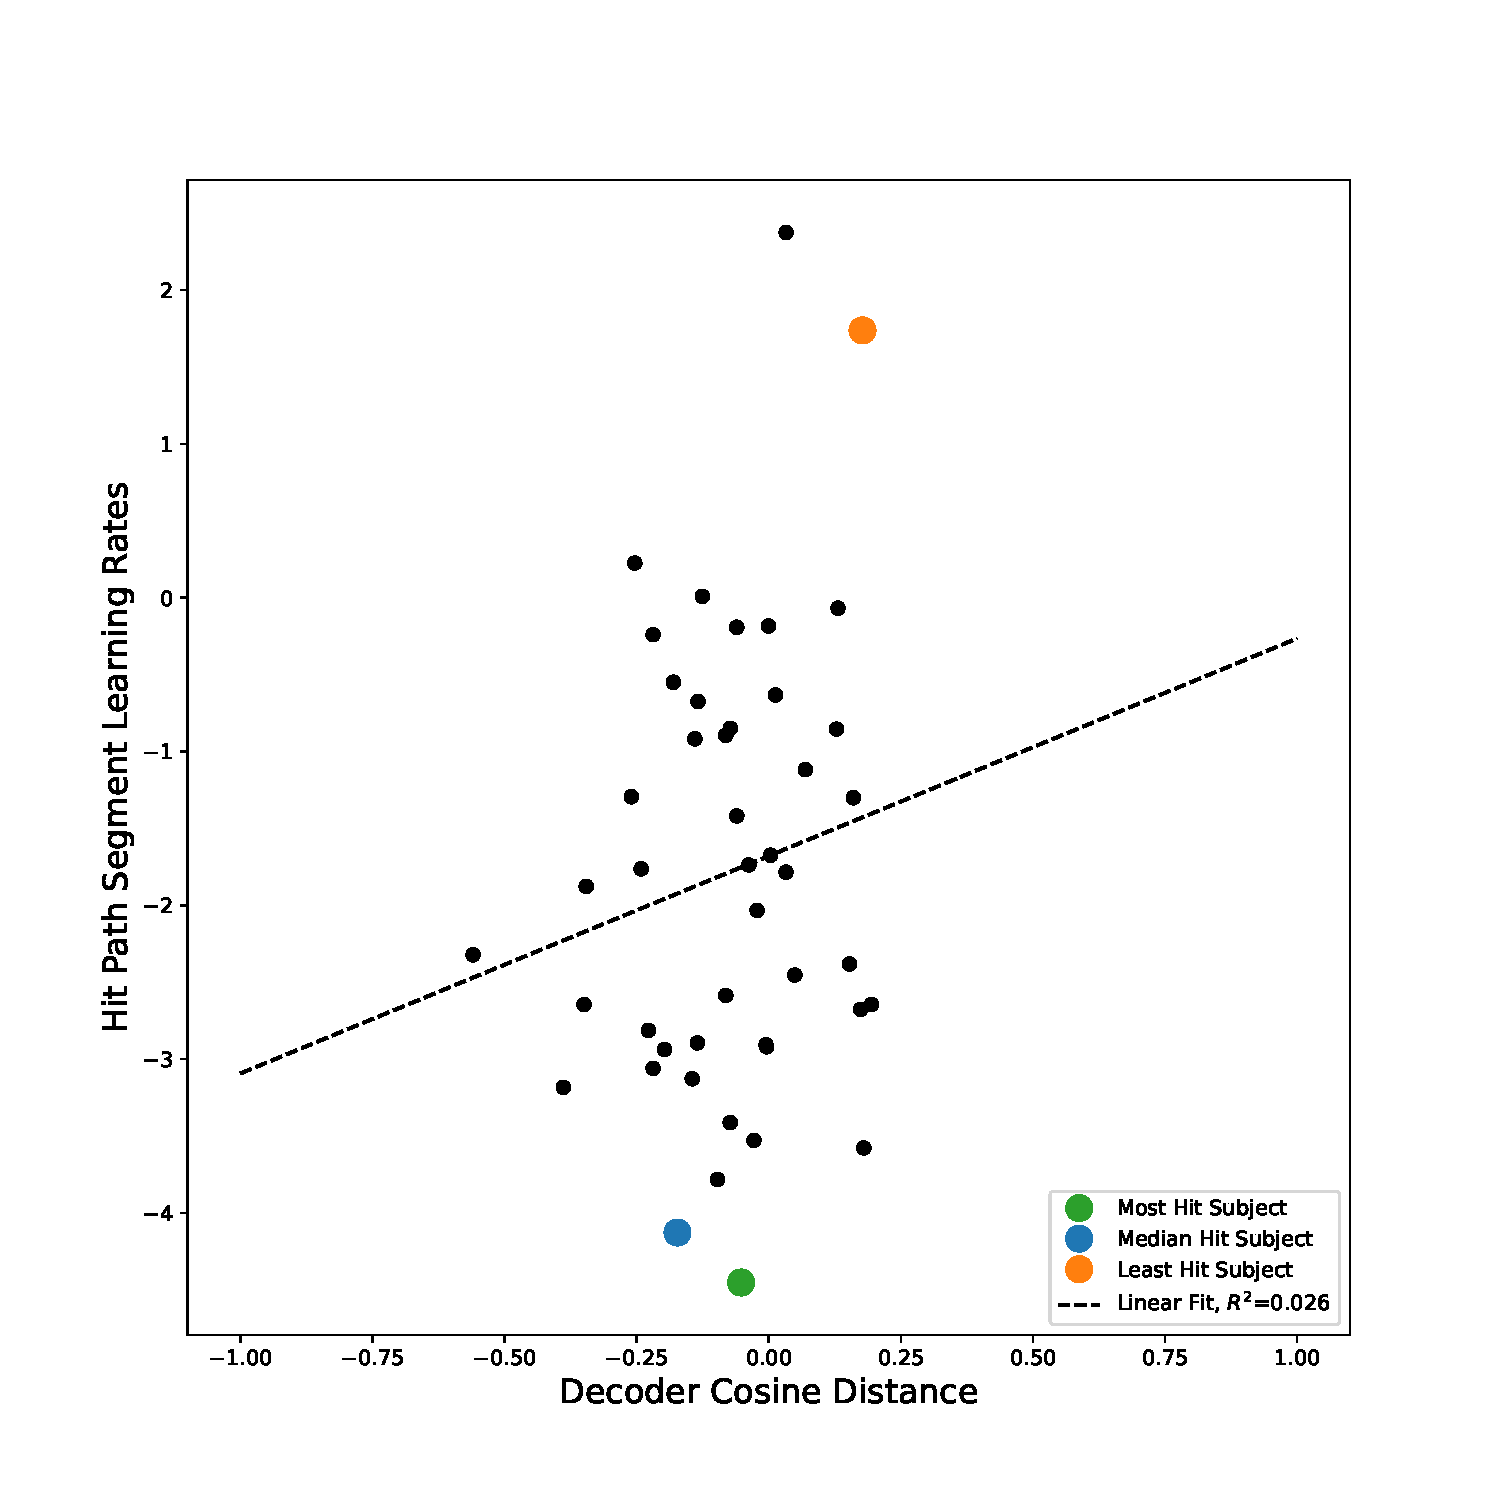
\includegraphics[width=\textwidth]{analysis/segment_lr_decoder_cosine.pdf}
%             \caption{}            
%             \label{fig:path_length_learning_rates}
%         \end{subfigure}%
%     }
%     \caption{Learning rates for different measures of performance}
%     \label{fig:three graphs}
% \end{figure}

\cleardoublepage\printendnotes%
\ifSubfilesClassLoaded{%
    \newpage%
    \bibliography{../bib/bibliography}%
}{}%
\end{document}